% article example for classicthesis.sty
\documentclass[10pt,a4paper]{article} % KOMA-Script article scrartcl
\usepackage{lipsum}
\usepackage{url}
\usepackage[nochapters]{classicthesis} % nochapters
\usepackage{polski}
\usepackage[utf8]{inputenc}
\usepackage{enumerate}
\usepackage{float}
\usepackage{subcaption}
\usepackage{graphicx}
\usepackage{amsmath}
\usepackage[T1]{fontenc}

\begin{document}
    \pagestyle{plain}
    \title{\rmfamily\normalfont\spacedallcaps{Opracowanie zagadnień na egzamin dyplomowy}}
    \date{} % no date

    \maketitle

    \tableofcontents

    \section{Zagadnienia obejmujące podstawowe treści programowe kierunku studiów Fizyka Techniczna do egzaminu dyplomowego na studiach II stopnia}
    \subsection{Ruch w mechanice newtonowskiej i relatywistycznej}
    
\begin{enumerate}[1]
\item \underline{Zasada dynamiki Newtona:}

I zasada dynamiki Newtona zakłada istnienie inercjalnego układu odniesienia. Układ inercjalny to taki, w którym cząstka nie podlegająca oddziaływaniu z otoczeniem, spoczywa lub porusza się po prostej ze stałą predkością (układy inercjalne poruszają się ruchem jednostajnym lub spoczywają względem siebie).

\item \underline{Zasada dynamiki Newtona:}
	
W inercjalnym układzie odniesienia jeśli siły działające na ciało nie rownoważą się ($ \vec{F_w} \neq 0 $) to ciało porusza się z przyśpieszeniem wprost proporcjonalnym do siły wypadkowej, a odwrotnie proporcjonalnym do masy ciała:\newline
$ \vec{a} = \frac{1}{m}*\vec{F_w} $\newline
$ \vec{F_w} = \frac{d\vec{p}}{dt} = \frac{d}{dt}(m\vec{v}) = m\frac{d\vec{v}}{dt} = m\vec{a} $\newline
Pierwsza zasada dynamiki Newtona jest szczególnym przypadkiem drugiej zasady dynamiki Newtona (gdy $ \vec{F_w} = 0 $).

\item \underline{Zasada dynamiki Newtona:}

Oddziaływania ciał są zawsze wzajemne. Jeżeli ciało \textit{A} działa na ciało \textit{B} siła $\vec{F}$ (akcja), to ciało \textit{B} działa na ciało \textit{A} siłą o takiej samej wartości i kierunku, lecz przeciwnym zwrocie (reakcja).
	
\end{enumerate}

\underline{Szczególna teoria względności}

\begin{enumerate}[1]
	\item \underline{postulat}:
	
We wszystkich układach inercjalnych prawa fizyki są jednakowe (zasada względności).

	\item \underline{postulat}:
	
Dla wszystkich obserwatorów inercjalnych prędkość światła w próżni (\textit{c}) jest taka sama i nie zależy od prędkości źródła światła.

\end{enumerate}

Te postualaty Einsteina prowadzą do tranformacji Lorentza:\newline
Rozważmy układ K oraz układ K' poruszający się względem K z predkością $ v_x $ wzdłuż osi OX (dla t = t' = 0 początki układów współrzednych $ 0_K $ i $ 0_{K'} $ pokrywają się), wtedy:\newline
$ t' = \gamma(\textit{t} - \frac{v_xx}{c^2}) $, $\gamma = \frac{1}{\sqrt{1-\frac{v_x^2}{c^2}}}$\newline
$ x'=\gamma(x - v_xt) $, y'=y, z'=z

Konsekwencje szczególnej teorii względności:

\begin{enumerate}[-]
\item Względność jednoczesności - dwa zdarzenia określone przez jednego obserwatora jako jednoczesne, mogą nie być jednoczesne dla innego obserwatora.
\item Dylatacja czasu - czas, jaki mija pomiędzy dwoma zdarzeniami, nie jest jednoznacznie określony, lecz zależy od ruchu obserwatora (paradoks bliźniąt).
\item Relatywistyczne składanie prędkości.
\item Masa jest równoważna energii $ E=mc^2 $.
\item Ciała bezmasowe poruszają się z prędkością c, dla ciał z niezerową masą niemożliwe jest osiągnięcie prędkości c.
\item Skrócenie Lorentza.
\end{enumerate}
    \subsection{Zasady zachowania i symetrie w fizyce}
	Jeśli układ posiada pewną symetrię, oznacza to, że równania opisujące ten układ nie zmieniają swojej postaci po dokonaniu przekształceń symetrii.

\underline{Dyskretne przekształcenia symetrii} to takie, których nie można sparametryzować np.
\begin{enumerate}[-]
	
\item Teoria grup i symetrii translacyjnej dla sieci periodycznej w kryształach.
\item Symetria permutacyjna funkcji falowej dla układu wielu ciał - związana z nierozróżnialnością cząstek elementarnych (zamiana miejscami cząstek układu nie zmiłaby równań opisujących układ).
\item Symetria zwierciadlana \textbf{P} związana z przekształceniem odbicia przestrzennego (zmiana znaków składowych przestrzennych wektorów na przeciwne).
\item Odwracalność w czasie \textbf{T} (zmiana znaku czasu w równaniach).
\item Parzystość ładunkowa \textbf{C} (zmiana znaku ładunku).

\end{enumerate}

Elektromagnetyzm, grawitacja i oddziaływania silne są niezmiennicze względem każdej z ostatnich trzech wymienionych symetrii (CPT) osobno, jednakże w przypadku oddziaływań słabych niezmienniczość jest zachowana tylko w przypadku łącznego ich działania CPT (rozpad $ \beta $ łamie symetrie P i C, ale zachowuje połączoną symetrie CP, która dla odmiany jest łamana w przypadku rozpadu mezonów K).

\underline{Symetrie związane z ciągłymi przekształceniami} są bezpośrednio związane z istnieniem zasad zachowania - związek ten opisuje twierdzenie Noether. Zgodnie z tym twierdzeniem, z daną symetrią układu jest związanych tyle praw zachowania, ile ciągłych rzeczywistych parametrów potrzebnych jest do sparametryzowania odpowiadających tej symetrii przekształceń np.

\begin{enumerate}[-]
\item Zasada zachowania energii wynika z symetrii związanej z przesunięciem w czasie - niezmienniczości działania S opisującego ruch danego układu od czasu (t - parametr). Jeżeli układ absorbuje lub emituje energie, wówcząs to działanie jest funkcją czasu (t) - odpowiada to w konsekwencji zmianie energii układu.

\item Zasada zachowania pędu wynika z symetrii związanej z przesunięciem układu w przestrzeni.

\item Zasada zachowania momentu pędu wynika z z symetrii związanej z obrotem układu.

\item Zasada zachowania ładunku wyniki z niezmienniczości funkcji falowej elektronu względem transformacji cechowania.
\end{enumerate}
	\subsection{Klasyczny i kwantowy oscylator harmoniczny}
	Lalala
	\subsection{Fizyczna treść równań Maxwella i równania falowego.}
	\begin{figure} [H]
	\centering
	\begin{subfigure}{.49\textwidth}
		\centering
		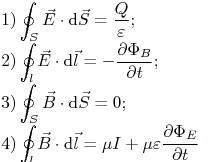
\includegraphics[width=1.0\linewidth]{generalIssues/Figures/maxwell1.png}
		\caption{Postać całkowa.}
		\label{n1}
	\end{subfigure}
	\begin{subfigure}{.49\textwidth}
		\centering
		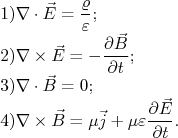
\includegraphics[width=1.0\linewidth]{generalIssues/Figures/maxwell2.png}
		\caption{Postać różniczkowa.}
		\label{r1}
	\end{subfigure}
	\caption{Równania Maxwella.}
	\label{maxwell}
\end{figure}

Rysunek~\ref{maxwell} przedstawia równania Maxwella, gdzie:\newline
$ \varrho $ - gęstość ładunku,\newline
$ \varepsilon $ - przenikalność dielektryczna,\newline
$ \mu $ - przenikalność magnetyczna,\newline
$ \vec{j} $ - gęstość prądu,\newline
$ \Phi_B $- strumień indukcji magnetycznej,\newline
$ \Phi_E $- strumień natężenia pola elektrycznego,\newline
$ \nabla * \vec{F} = \frac{\partial F_x(x,y,z)}{\partial x} + \frac{\partial F_y(x,y,z)}{\partial y} + \frac{\partial F_z(x,y,z)}{\partial z}$ - dywergencja pola wektorowego $ \vec{F} = [F_x, F_y, F_z] $,\newline
$
\nabla \times \vec{F} = 
\begin{vmatrix}
\textbf{i} & \textbf{j} & \textbf{k} \\ 
\frac{\partial}{\partial x} & \frac{\partial}{\partial y} & \frac{\partial}{\partial z} \\ 
F_x & F_y & F_z  \notag
\end{vmatrix}
= (\frac{\partial F_z}{\partial y} - \frac{\partial F_y}{\partial z})\textbf{i} + (\frac{\partial F_x}{\partial z} - \frac{\partial F_z}{\partial x})\textbf{j} + (\frac{\partial F_y}{\partial x} - \frac{\partial F_x}{\partial y})\textbf{k}
$ - rotacja pola wektorowego $ \vec{F} $.\newline

Sens fizyczny praw Maxwella:
\begin{enumerate}[1)]
	\item \underline{Prawo Gaussa dla elektryczności} - źródłem pola elektrycznego są ładunki, a strumień tego pola przez dowolną powierzchnię zamkniętą zależy tylko od ładunku zamkniętego przez tę powierzchnię.
	\item \underline{Prawo Faradaya} - zmiana strumienia indukcji magnetycznej przez powierzchnię zamkniętej pętli powoduje powstanie w tej pętli siły elektromotorycznej indukcji (SEM), a kierunek płynącego prądu jest taki, żeby przeciwdziałać zmianom powodującym indukcję (reguła Lenza).
	\item \underline{Prawo Gaussa dla magnetyzmu} - nie istnieją ładunki magnetyczne, a strumień pola magnetycznego przez dowolną powierzchnię zamkniętą jest równy 0.
	\item \underline{Prawo Ampere'a} - zmienne pole elektryczne i płynący prąd powodują powstanie pola magnetycznego.
\end{enumerate}

Dla fali elektromagnetycznej w próżni wektory $ \vec{E} $ i $ \vec{B} $ drgają w płaszczyznach wzajemnie prostopadłych i dla fali rozchodzącej się w kierunku osi x możemy przyjąć taki układ odniesienia aby wektor $ \vec{E} $ drgał w kierunku osi y a wektor $ \vec{B} $ w kierunku osi z. Zatem wektory $ \vec{E} $ i $ \vec{B} $ mają tylko po jednej składowej:\newline
$ \vec{E} = [0, E, 0] $,\newline
$ \vec{B} = [0, 0, B] $.\newline
Liczmy rotację wektorów $ \vec{E} $ i $ \vec{B} $ (wykorzystując fakt, że nasza fala jest falą płaską i pola $ \vec{E} $ i $ \vec{B} $ zmieniają się tylko względem współrzędnej x, czyli że $ \frac{\partial E}{\partial z} = 0, \frac{\partial B}{\partial y} = 0$):\newline
$ \nabla \times \vec{E} = \textbf{k}\frac{\partial E}{\partial x} $,\newline
$ \nabla \times \vec{B} = -\textbf{j}\frac{\partial B}{\partial x} $.\newline

Korzystając z równań Faradaya oraz Ampera w postaci różniczkowej otrzymujemy (poszukujemy równania dla fal elektromagnetycznych rozchodzących się w próżni gdzie nie będą występowały prądy przewodzenia, czyli $ \vec{j} $ = 0):\newline
$ \textbf{k}\frac{\partial E}{\partial x} = -\frac{\partial \vec{B}}{\partial t} = -\textbf{k}\frac{\partial B}{\partial t} $,\newline
$ \textbf{j}\frac{\partial B}{\partial x} = -\mu_0 \epsilon_0 \frac{\partial \vec{E}}{\partial t} = -\textbf{j} \mu_0 \epsilon_0 \frac{\partial E}{\partial t} $.\newline
W efekcie dostajemy układ dwóch równań:\newline
$ \frac{\partial E}{\partial x} = -\frac{\partial B}{\partial t} $,\newline
$ \frac{\partial B}{\partial x} = - \mu_0 \epsilon_0 \frac{\partial E}{\partial t} $.\newline

Równania falowe dla $ \vec{E} $ i $ \vec{B} $ będą miały identyczną postać. Jeżeli zdecydujemy się szukać równania dla $ \vec{E} $, to eliminujemy z naszego układu równań $ \vec{B} $ przez utworzenie pochodnych mieszanych $ \vec{E} $ względem x i t. Różniczkujemy zatem pierwsze równanie po x, a drugie po t (jeśli chcemy szukać równania dla $ \vec{B} $ eliminujemy w ten sam sposób z naszych równań $ \vec{E} $):\newline
$ \frac{\partial^2 E}{\partial x^2} = -\frac{\partial^2 B}{\partial t \partial x} $,\newline
$ \frac{\partial^2 B}{\partial t \partial x} = - \mu_0 \epsilon_0 \frac{\partial^2 E}{\partial t^2} $.\newline
Z powyższego układu równań otrzymujemy poszukiwane równanie falowe dla pola $ \vec{E} $:\newline
$ \frac{\partial^2 E}{\partial x^2} - \mu_0 \epsilon_0 \frac{\partial^2 E}{\partial t^2} = 0 $\newline
Znając ogólną postać równania falowego dla fali rozchodzącej się z predkością v w kierunku osi x:\newline
$ \frac{\partial^2 \xi}{\partial x^2} - \frac{1}{v^2} \frac{\partial^2 \xi}{\partial t^2} = 0 $\newline
otrzymujemy związek pomiędzy prędkością światła w próżni (c) a wartościami przenikalności elektrycznej i magnetycznej próżni: \newline
$ c = \frac{1}{\sqrt{\mu_0 \epsilon_0}} $.\newline
Rozwiązanie równania falowego dla pola $ \vec{E} $ ma postać:\newline
$ \vec{E} = \vec{E_0}\sin(kx - \omega t) $,\newline
gdzie: $ k = \frac{2\pi}{\lambda} $, $ \omega = ck $.
	
	\subsection{Właściwości fal elektromagnetycznych.}
	Falą elektromagnetyczną nazywamy rozchodzące się w przestrzeni zaburzenie pola elektromagnetycznego. Składowa elektryczna i magnetyczna fali indukują się wzajemnie – zmieniające się pole elektryczne wytwarza zmieniające się pole magnetyczne, a z kolei zmieniające się pole magnetyczne wytwarza zmienne pole elektryczne.

Promieniowanie elektromagnetyczne przejawia właściwości falowe ulegając interferencji, dyfrakcji, spełnia prawo odbicia i załamania. W wyniku superpozycji fal elektromagnetycznych może powstać fala stojąca. 

Strumień energii przenoszonej przez falę elektromagnetyczną w każdym punkcie przestrzeni określa wektor Poyntinga zdefiniowany jako:\newline
$ \vec{S} = \frac{1}{\mu_0} \vec{E} \times \vec{B} $,\newline
gdzie:\newline
$ \mu_0 $ - przenikalność magnetyczna próżni,\newline
$ \vec{E} $ - natężenie pola elektrycznego,\newline
$ \vec{B} $ - indukcja pola magnetycznego.

Choć w elektrodynamice klasycznej energię promieniowania elektromagnetycznego uważa się za wielkość ciągłą, zależną jedynie od natężenia pola elektrycznego i indukcji pola magnetycznego, to zjawiska zachodzące na poziomie atomowym dowodzą, że jest ona skwantowana. Energia pojedynczego kwantu jest zależna tylko od częstotliwości fali $ \nu $ i wynosi:\newline
$ E = h \nu $, gdzie \textit{h} - stała Plancka.

Właściwości fal elektromagnetycznych zależą od długości fali. Promieniowaniem elektromagnetycznym o różnej długości fali są:
 
\begin{enumerate}[-]
	\item \underline{Fale radiowe} (długość fali powyżej 1 m) - znajdują bardzo szerokie zastosowanie w telekomunikacji, radiofonii, telewizji, radioastronomii i wielu innych dziedzinach nauki i techniki. Naturalne źródła fal radiowych to między innymi wyładowania atmosferyczne, zorze polarne, radiogalaktyki.
	\item \underline{Mikrofale} (od 1 mm do 1 m) - podstawowe zastosowania mikrofal to łączność (na przykład telefonia komórkowa, radiolinie, bezprzewodowe sieci komputerowe) oraz technika radarowa. Fale zakresu mikrofalowego są również wykorzystywane w radioastronomii, a odkrycie mikrofalowego promieniowania tła miało ważne znaczenie dla rozwoju i weryfikacji modeli kosmologicznych. Wiele dielektryków mocno absorbuje mikrofale, co powoduje ich rozgrzewanie i jest wykorzystywane w kuchenkach mikrofalowych, przemysłowych urządzeniach grzejnych i w medycynie.
	\item \underline{Podczerwień} (od 700 nm do 1 mm) - promieniowanie podczerwone jest nazywane również cieplnym, szczególnie gdy jego źródłem są nagrzane ciała. Każde ciało o temperaturze większej od zera bezwzględnego emituje takie promieniowanie, a ciała o temperaturze pokojowej najwięcej promieniowania emitują w zakresie długości fali rzędu 10 $ \mu m $. Przedmioty o wyższej temperaturze emitują promieniowanie o większym natężeniu i mniejszej długości, co pozwala na zdalny pomiar ich temperatury i obserwację za pomocą urządzeń rejestrujących wysyłane promieniowanie (termowizja).
	\item \underline{Światło widzialne} (od 380 nm do 700 nm) - światło (promieniowanie widzialne) to ta część widma promieniowania elektromagnetycznego, na którą reaguje zmysł wzroku człowieka. Różne zwierzęta mogą widzieć w nieco różnych zakresach. Światło ma bardzo duże znaczenie w nauce i wiele zastosowań w technice. Dziedziny nauki i techniki zajmujące się światłem noszą nazwę optyki.
	\item \underline{Ultrafiolet} (od 10 nm do 380 nm) - promieniowanie ultrafioletowe jest zaliczane do promieniowania jonizującego, czyli ma zdolność odrywania elektronów od atomów i cząsteczek. W technice ultrafiolet stosowany jest powszechnie. Powoduje świecenie (fluorescencję) wielu substancji chemicznych. W świetlówkach ultrafiolet wytworzony na skutek wyładowania jarzeniowego pobudza luminofor do świecenia w zakresie widzialnym. Niektóre owady, na przykład pszczoły, widzą w bliskiej światłu widzialnemu części widma promieniowania ultrafioletowego, również rośliny posiadają receptory ultrafioletu. 
	\item \underline{Promieniowanie rentgenowskie} (od 5 pm do 10 nm) - promieniowanie rentgenowskie jest promieniowaniem jonizującym. Technicznie promieniowanie rentgenowskie uzyskuje się przeważnie poprzez wyhamowywanie rozpędzonych cząstek naładowanych. W lampach rentgenowskich są to rozpędzone za pomocą wysokiego napięcia elektrony hamowane na metalowych anodach. Źródłem wysokoenergetycznego promieniowania rentgenowskiego są również przyspieszane w akceleratorach cząstki naładowane. Promieniowanie rentgenowskie jest wykorzystywane do wykonywania zdjęć rentgenowskich do celów defektoskopii i diagnostyki medycznej. W zakresie promieniowania rentgenowskiego są również prowadzone obserwacje astronomiczne. 
	\item \underline{Promieniowanie gamma} (0,03 pm do 300 pm) - promieniowania gamma jest promieniowaniem jonizującym. Promieniowanie gamma towarzyszy reakcjom jądrowym, powstaje w wyniku anihilacji – zderzenie cząstki i antycząstki, oraz rozpadów cząstek elementarnych. Otrzymywane w cyklotronach promieniowanie hamowania i synchrotronowe również leży w zakresie długości fali promieniowania gamma, choć niekiedy bywa nazywane wysokoenergetycznym promieniowaniem rentgenowskim. Promienie gamma mogą służyć do sterylizacji żywności i sprzętu medycznego. W medycynie używa się ich w radioterapii oraz w diagnostyce. Zastosowanie w przemyśle obejmują badania defektoskopowe. Astronomia promieniowania gamma zajmuje się obserwacjami w tym zakresie długości fal. 
\end{enumerate}
	
	\subsection{Interferencja i dyfrakcja fal.}
	\underline{Interferencja} jest to zjawisko powstawania nowego, przestrzennego rozkładu amplitudy fali (wzmocnienia i wygaszenia) w wyniku nakładania się (superpozycji fal) dwóch lub więcej fal. Warunkiem trwałej interferencji fal jest ich spójność, czyli korelacja faz i równość częstotliwości. 

Dla najprostszego przypadku dwóch fal harmonicznych o jednakowych amplitudach A, jednakowej długości fali $ \lambda $ i zgodnych fazach początkowych, rozchodzących się z dwóch różnych źródeł, które leżą w odległościach odpowiednio $ d_1 $ i $ d_2 $ od punktu P, zaburzenie w punkcie P opisuje wzór:\newline
$ y(P) = A\sin (\omega t + \phi_1) + A\sin (\omega t + \phi_2)$, gdzie:\newline
$ \phi_1 = 2\pi\frac{d_1}{\lambda} $,\newline
$ \phi_2 = 2\pi\frac{d_2}{\lambda} $.\newline
Gdy spełniony jest warunek:\newline
$ \phi_1 - \phi_2 = 2\pi\frac{d_1-d_2}{\lambda} = 2k\pi $,\newline
gdzie k - dowolna liczba naturalna, to fale w punkcie P ulegają wzmocnieniu (są w tej samej fazie) i:\newline
$ y(P) = 2A\sin (\omega t) $.\newline
Gdy natomiast w pewnym punkcie $ P_1 $:\newline
$ \phi_1 - \phi_2 = 2\pi\frac{d_1-d_2}{\lambda} = (2k+1)\pi $\newline
wtedy fale wygaszają się (są w przeciwfazie) i:\newline
$ y(P_1) = 0 $.

Interferencja pozwala na bardzo precyzyjny pomiar zmian długości drogi od źródła do detektora fali.

\underline{Dyfrakcja} (ugięcie fali) – zespół zjawisk związanych ze zmianą kierunku rozchodzenia się fali będący odstępstwem od praw optyki geometrycznej (dział optyki zajmujący się wytłumaczeniem zjawisk optycznych przy użyciu pojęcia promienia). Dyfrakcję w węższym znaczeniu określa się jako ugięcie światła wokół krawędzi przeszkody lub otworu w obszarze cienia przeszkody.

Zjawisko dyfrakcji rozpatruje się jako interferencję fal cząstkowych powstających zgodnie z zasadą Huygensa. Jest to zasada stosowana do określenia rozchodzenia się fali w ośrodku, mówiąca, iż każdy punkt ośrodka, do którego dotarło czoło fali, można uważać za źródło nowej fali kulistej. Wypadkową powierzchnię falową tworzy powierzchnia styczna do wszystkich powierzchni fal cząstkowych i ją właśnie obserwuje się w ośrodku.

Rysunek~\ref{diffracion} przedstawia dyfrakcję na pojedynczej szczelinie. Gdy różnica dróg fali ze skrajnego i środkowego elementu równa jest połowie długości fali, to fale z obu połówek szczeliny wygaszą się. Jeżeli wiązki są niemal równoległe, to różnica odległości pojawia się tylko przy wyjściu promieni ze szczeliny, wówczas:\newline
$ d\sin(\theta_{min}) = \lambda $.\newline

Przepuszczenie fali przez szczelinę dyfrakcyjną pozwala na określenie kierunku rozchodzenia się fali. Im mniejsza jest szerokość szczeliny, tym dokładniej można to zrobić. Jednocześnie zmniejszanie szczeliny powoduje, że trudniej jest określić energię fali, ponieważ rozprasza się ona na większy obszar. W efekcie iloczyn błędu określenia energii oraz błędu pomiaru kierunku musi być większy od pewnej stałej. Oznacza to, że istnieje granica dokładności pomiaru parametrów rozchodzącej się fali. Próba dokładniejszego określenia jednego z parametrów fali powoduje zwiększenie niepewności pomiaru drugiego sprzężonego z nim. Zjawisko to ma fundamentalne znaczenie, jeżeli weźmie się pod uwagę, że każda materialna cząstka jest falą. Zjawisko to w mechanice kwantowej odpowiada zasadzie nieoznaczoności

\begin{figure} [H]
	\centering
	\begin{subfigure}{.99\textwidth}
		\centering
		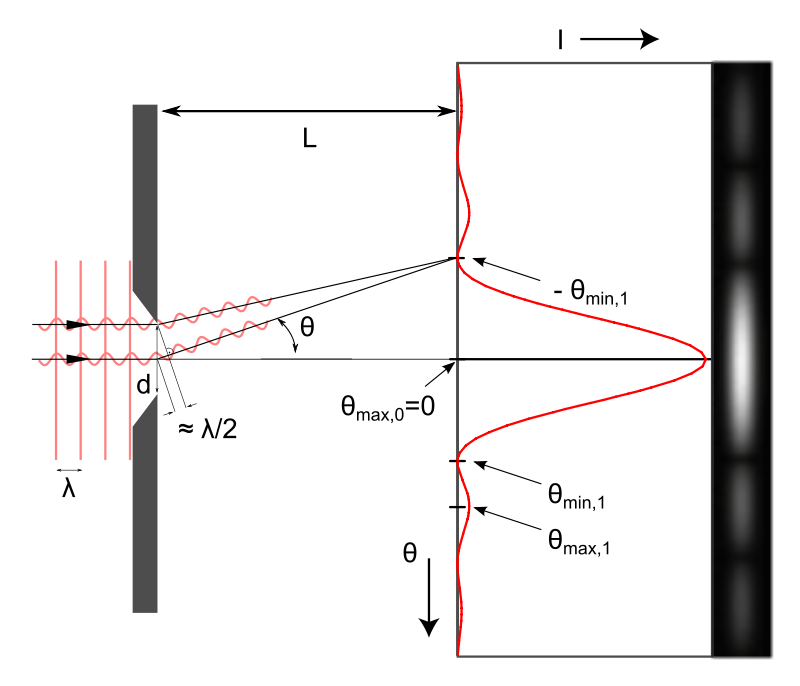
\includegraphics[width=0.6\linewidth]{generalIssues/Figures/diffraction.png}
	\end{subfigure}
	\caption{Dyfrakcja na pojedynczej szczelinie.}
	\label{diffracion}
\end{figure}

Pierwszą najprostszą formę eksperymentu przejścia światła przez podwójną szczelinę (rysunek~\ref{diffracion2}), zwaną obecnie doświadczenie Younga wykonał Thomas Young w 1801 roku. Eksperyment ten był zaczątkiem do uznania w XIX w falowej teorii światła. 

\begin{figure} [H]
	\centering
	\begin{subfigure}{.99\textwidth}
		\centering
		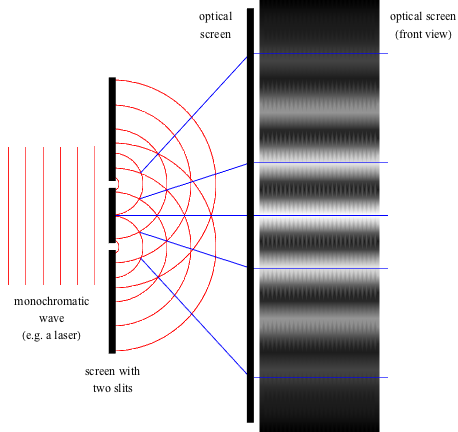
\includegraphics[width=0.6\linewidth]{generalIssues/Figures/diffraction2.png}
	\end{subfigure}
	\caption{Przejście światła przez podwójną szczelinę.}
	\label{diffracion2}
\end{figure}

Dla obrazów dyfrakcyjnych powstałych po przejściu światła przez otwór kołowy definiuje się \underline{warunek Rayleigha} określający zdolność rozdzielczą elementów i układów optycznych:\newline
$ \phi \approx \sin(\phi) = 1.22 \frac{\lambda}{d} $ (przybliżenie dla małych kątów), gdzie:\newline
$ \phi $ - minimalny kąt między promieniami, których obrazy mają być rozróżnialne, czyli inaczej – ich odległość kątowa,\newline
$ \lambda $ - długość fali światła,\newline
$ d $ - średnica otworu.\newline

Aby wzmocnić falę przechodzącą przez szczelinę stosuje się w optyce układy wielu takich szczelin, nazywane \underline{siatką dyfrakcyjną} (rysunek~\ref{diffracion3}). Efekty optyczne od każdej szczeliny dodają się, przez co zachowanie fali zależy tylko od stałej siatki (odległości dzielącej najbliższe sobie rysy). Zjawisko dyfrakcji zachodzi również, kiedy fale przechodzą przez wiele blisko siebie położonych warstw. Jeżeli odległość między warstwami jest stała, kolejne maksima fali można opisać zależnością:\newline
$ \sin(\theta) = \frac{n\lambda}{d} $, gdzie:\newline
$ d $ - stała siatki,\newline
$ \theta $ - kąt od osi wiązki światła,\newline
$ \lambda $ - długość fali,\newline
$ d $ - przyjmuje wartości całkowite dodatnie od 1,2,3,...\newline

\begin{figure} [H]
	\centering
	\begin{subfigure}{.99\textwidth}
		\centering
		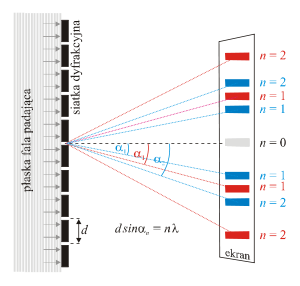
\includegraphics[width=0.6\linewidth]{generalIssues/Figures/diffraction3.png}
	\end{subfigure}
	\caption{Siatka dyfrakcyjna.}
	\label{diffracion3}
\end{figure}

Zjawisko dyfrakcji pozwoliło na rozwój krystalografii rentgenowskiej, dzięki której badano strukturę kryształów, odkryto w ten sposób także strukturę spirali DNA. 
	
	\subsection{Zasady termodynamiki.}
	\underline{Zerowa zasada termodynamiki} - jeśli układy A i B mogące ze sobą wymieniać ciepło si ą ze sobą w równowadze termicznej, i to samo jest prawdą dla układów B i C, to układy A i C również są ze sobą w równowadze termicznej. Z zasady tej wynika istnienie temperatury empirycznej. Temperatura to taka wielkość fizyczna, która dla układów A, B i C jest równa, gdy ustaje przepływ ciepła. Układy będą ze sobą w równowadze termodynamicznej. Zerowa zasada termodynamiki stwierdza także, że ciało w równowadze termodynamicznej ma wszędzie tę samą temperaturę.

\underline{Pierwsza zasada termodynamiki} - zmiana energii wewnętrznej (będącej funkcją stanu) układu zamkniętego (nie wymienia masy z otoczeniem) jest równa energii, która przepływa przez jego granice na sposób ciepła i pracy:\newline
$ \Delta U = W + Q $, gdzie:\newline
$ \Delta U $ - zmiana energii wewnętrznej układu,\newline
$ W $ - praca wykonana na układzie,\newline
$ Q $ - ciepło przekazane do układu.\newline
Alternatywne sformułowanie - nie istnieje perpetuum mobile pierwszego rodzaju (maszyna, która wytwarza więcej energii, niż sama zużywa).

\underline{Druga zasada termodynamiki} - w układzie termodynamicznie izolowanym istnieje funkcja stanu zwana entropią, która nie maleje z czasem. Matematyczny zapis tego faktu to następujące sformułowanie: zmiana entropii $ \Delta S $ w dowolnym procesie odwracalnym jest równa całce z przekazu ciepła DQ podzielonego przez temperaturę T. W procesie nieodwracalnym natomiast zmiana entropii jest większa od tej całki:
$ \Delta S \geq \int \frac{DQ}{T} $\newline
Różnica ta jest miarą nieodwracalności procesu i jest związana z rozpraszaniem energii. Entropia (S) jest funkcją stanu będąca miarą liczby sposobów (W), na jakie może być zrealizowany określony stan termodynamiczny danego układu w określonej temperaturze (T). Układ dąży do stanu, który może być w danych warunkach zrealizowany na jak najwięcej sposobów; dąży więc on do maksymalizacji entropii. Nie można bez wkładu pracy przesyłać energii termicznej między ciałami mającymi tę samą temperaturę. Oznacza to, że perpetuum mobile drugiego rodzaju (maszyna, która zamienia energię cieplną na pracę mechaniczną bez wzrostu całkowitej entropii) nie istnieje. 

\underline{Trzecia zasada termodynamiki} - nie można za pomocą skończonej liczby kroków uzyskać temperatury zera bezwzględnego (zero kelwinów), jeżeli za punkt wyjścia obierzemy niezerową temperaturę bezwzględną. Podstawą takiego zdefiniowania III zasady termodynamiki jest analiza sprawności lodówki. Jak wiemy, lodówka działa na zasadzie odwrotnego cyklu Carnota, a jej sprawność dana jest wzorem:\newline
$ n = \frac{Q_{odebrane}}{W} = \frac{T_2}{T_1-T_2} $\newline
Jeżeli ciało o określonej temperaturze $ T_1 $ chcielibyśmy schłodzić do $ T_2 \to $, odbierając przy tym skończone ciepło $ Q $, to analizując wzór widzimy, że w takim wypadku $ \frac{Q}{W} \to 0 $, czyli $ W\to $ nieskończoności. Gdybyśmy podstawili $ T_2 = 0 $, równanie nie miałoby sensu matematycznego, co oznacza, że nie da się osiągnąć temperatury zera bezwzględnego w skończonej liczbie kroków. Mówiąc inaczej, gdyby udało się schłodzić jakąś substancję do 0 K i gdyby utworzyła ona kryształ doskonały nieposiadający zamrożonych defektów krystalicznych, to jej entropia musiałaby przyjąć wartość 0. Jest to jednak technicznie, a także formalnie, niewykonalne:
$ \lim_{T\to0} S = 0 $
	
	\subsection{Entropia w ujęciu termodynamicznym i statystycznym.}
	Entropia jest to termodynamiczna funkcja stanu, określająca kierunek przebiegu procesów spontanicznych (samorzutnych) w odosobnionym układzie termodynamicznym. Entropia jest miarą stopnia nieuporządkowania układu i rozproszenia energii. Jest wielkością ekstensywną. Zgodnie z drugą zasadą termodynamiki, jeżeli układ termodynamiczny przechodzi od jednego stanu równowagi do drugiego, bez udziału czynników zewnętrznych (a więc spontanicznie), to jego entropia zawsze rośnie. W ramach II zasady termodynamiki zmiana entropii (w procesach kwazistatycznych) jest zdefiniowana przez swoją różniczkę zupełną jako:\newline
$ dS = \frac{1}{T}\delta Q $, gdzie:\newline
$ T $ - temperatura bezwzględna,\newline
$ \delta Q $ - ciepło elementarne, czyli niewielka ilość ciepła dostarczonego do układu.\newline
Entropię pewnego stanu termodynamicznego P można wyznaczyć ze wzoru:\newline
$ S(P) = \int_{0}^{T_p}\frac{C(T)dT}{T} $, gdzie:\newline
$ C(T) $ - pojemność cieplna (ilość ciepła, jaka jest niezbędna do zmiany temperatury ciała o jednostkę temperatury),\newline
$ T_p $ - temperatura w stanie P.
Podstawowe równanie termodynamiki fenomenologicznej, w którym występuje entropia, ma postać:\newline
$ dU = TdS - pdV + \sum_{i=1}^{k}\mu_idN_i $, gdzie:\newline
$ U $ - energia wewnętrzna,\newline
$ k $ - liczba różnych składników,\newline
$ T $ - temperatura,\newline
$ p $ - ciśnienie,\newline
$ \mu_i $ - potencjał chemiczny i-tego składnika.

W termodynamice statystycznej całkowita entropia układu makroskopowego jest równa:\newline
$ S = k\ln(W) $\newline
lub\newline
$ S = -k\sum_{i}p_i\ln(p_i) $, gdzie:\newline
$ k $ - stała Boltzmanna,\newline
$ W $ - liczba sposobów, na jakie makroskopowy stan termodynamiczny układu (makrostan) może być zrealizowany poprzez stany mikroskopowe (mikrostany),\newline
$ p_i $ - prawdopodobieństwo i-tego mikrostanu.\newline
Zatem $ \log_2(W) $ jest liczbą bitów potrzebnych do określenia, którą realizację przyjął dany układ.


	
	\subsection{Klasyczne i kwantowe rozkłady statystyczne.}
	\underline{Gaz doskonały} - zwany też gazem idealnym, jest to abstrakcyjny, matematyczny model fizyczny gazu, spełniający następujące warunki: 

\begin{enumerate}[-]
	\item brak oddziaływań miedzycząsteczkowych z wyjątkiem odpychania w momencie zderzeń cząsteczek,
	\item objętość cząsteczek jest znikoma w stosunku do objętości gazu.
	\item zderzenia cząsteczek są doskonale sprężyste,
	\item cząsteczki znajdują się w ciągłym, chaotycznym ruchu.
\end{enumerate}

\underline{Rozkład Maxwella} – wzór określający rozkład prędkości cząstek gazu doskonałego. Założenie:  funkcja rozkładu f zależy tylko od wartości prędkości v:\newline
$ f(v_x,v_y,v_z) = f(v_x^2+v_y^2+v_z^2) $\newline
Żaden kierunek nie jest uprzywilejowany, ruch w każdym z kierunków x,y i z odbywa się niezależnie:\newline
$ f(v_x,v_y,v_z) = h(v_x)h(v_y)h(v_z) $\newline
Funkcja rozkładu h jest taka sama dla każdego kierunku co wynika z symetrii.\newline
$ ln[h(v_x)] + ln[h(v_y)] + ln[h(v_z)] = ln[f(v_x^2+v_y^2+v_z^2)] $, stąd:\newline
$ h(v_x) = C_xe^{(-Bv_x^2)} $\newline
$ f(v) = C_xC_yC_ze^{-B(v_x^2+v_y^2+v_z^2)} = Ce^{-Bv^2} $\newline
Stałą C znajdziemy z warunku normalizacji natomiast stałą B znajdujemy na podstawie równania łączącego średni kwadrat prędkości cząsteczek z temperaturą oraz wyrazić wartość średnią kwadratu prędkości poprzez funkcję gęstości prawdopodobieństwa:\newline
$ \frac{m<v^2>}{2} = \frac{3}{2}kT = \frac{m}{2}\int_{0}^{\infty} v^2f(v)*4\pi v^2dv $, gdzie:
$ m $ - masa cząsteczki,\newline
$ k $ - stała Boltzmanna,\newline
$ 4\pi v^2dv $ - element objętości przestrzeni prędkości (v, v+dv) we współrzędnych sferycznych.\newline
Otrzymujemy ostatecznie:\newline
$ f(v) = (\frac{m}{2\pi kT})^{\frac{3}{2}}e^{\frac{mv^2}{2kT}} $\newline
$ \frac{dP}{dv} = 4\pi (\frac{m}{2\pi kT})^{\frac{3}{2}}v^2e^{\frac{mv^2}{2kT}} $ - gęstość prawdopodobieństwa wystąpienia cząsteczki o prędkości v.\newline
Rozkład Maxwella pokazuje, że prędkości cząsteczek zależą od temperatury oraz masy molowej. Wraz ze wzrostem temperatury rozkład się poszerza (rysunek~\ref{maxwellDistribution}), a jego prędkość najbardziej prawdopodobna (tam gdzie dP/dv jest największe), jak i średnia prędkość (<v>) oraz średnia prędkość kwadratowa ($ \sqrt{<v^2>} $) zwiększają się.

\begin{figure} [H]
	\centering
	\begin{subfigure}{1.0\textwidth}
		\centering
		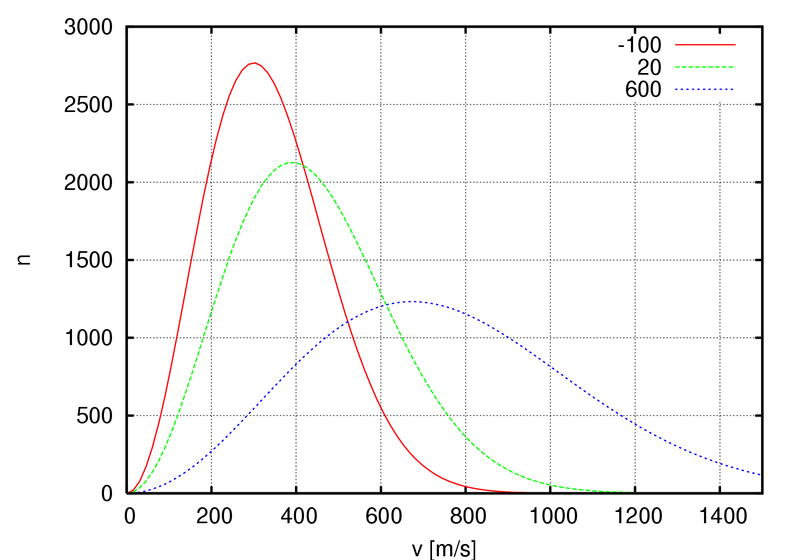
\includegraphics[width=0.98\linewidth]{generalIssues/Figures/maxwellDistribution.png}
	\end{subfigure}
	\caption{Rozkład Maxwella dla tlenu dla trzech temperatur (–100 $ ^\circ C $, temperatura pokojowa i 600 $ ^\circ C $). Wartość funkcji odpowiada liczbie cząsteczek spośród 1 miliona cząsteczek, jaka będzie poruszać się z prędkością v+/-0,5 m/s.}
	\label{maxwellDistribution}
\end{figure}

Wzór na koncentrację cząsteczek, czyli ich liczbę w jednostce objętości:\newline
$ n = n_0\exp(-\frac{E_p}{kT}) $, gdzie:\newline
$ E_p $ - energia potencjalna cząstek w danym stanie (np. na danej wysokości),\newline
$ n_0 $ - koncentracja cząsteczek dla $ E_p = 0 $ (np. koncentracja na powierzchni ziemi).\newline

Wzór ten wyraża zależność koncentracji cząsteczek od ich wysokości lub energii potencjalnej. Wynikający z niego rozkład koncentracji nosi nazwę rozkładu Boltzmanna i odnosi się nie tylko do pola sił przyciągania ziemskiego, ale do dowolnego pola potencjalnego, jeśli tylko cząsteczki poruszają się chaotycznym ruchem cieplnym. Liczba cząsteczek w objętości $ dV = dz \cdot dy \cdot dz $, której położenie określają współrzędne $ (x,y,z) $ wynosi:\newline
$ dn(x,y,z) = n_0\exp(-\frac{E_p(x,y,z)}{kT})dx\cdot dy\cdot dz $\newline
Nietrudno tu zauważyć podobieństwo rozkładów Maxwella i Boltzmanna, z tą różnicą, że pierwszy wyraża zależność od kwadratu prędkości lub energii kinetycznej, drugi - od energii potencjalnej. Rozkład zawierający obie te zależności nosi nazwę rozkładu Maxwella-Boltzmanna i ma postać:
$ dn(x,y,z,v_x,v_y,v_z) = A\exp(-\frac{E_p+E_k}{kt})dx\cdot dy \cdot dz \cdot v_x \cdot v_y \cdot v_z $

\underline{Zakaz Pauliego} głosi, że prawdopodobieństwo znalezienia w układzie fermionów (cząstek o spinie połówkowym) pary cząstek o jednakowych liczbach kwantowych jest równe zeru (czyli np. możemy znaleść na tej samej orbicie atomowej dwa elektrony, ale muszą mieć przeciwne spiny - jest to przykład degeneracji).

Zgodnie z rozkładem Fermiego-Diraca (rysunek~\ref{fermi})średnia liczba cząstek w niezdegenerowanym stanie energetycznym $ E $ dana jest przez:\newline

$ <n> = \dfrac{1}{e^{\beta (E-\mu)}+1} $, gdzie:\newline
$ E $ - energia tego stanu,\newline
$ \mu $ - potencjał chemiczny,\newline
$ \beta = 1/k_bT $\newline

\begin{figure} [H]
	\centering
	\begin{subfigure}{1.0\textwidth}
		\centering
		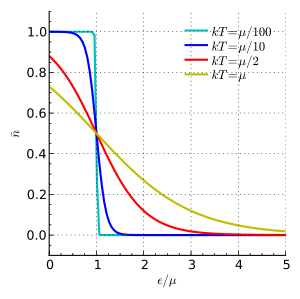
\includegraphics[width=0.7\linewidth]{generalIssues/Figures/fermi.png}
	\end{subfigure}
	\caption{Rozkład Fermiego-Diraca. Oś pozioma: $ E/\mu $. Oś pionowa: $ <n> $.}
	\label{fermi}
\end{figure}

W temperaturze zera bezwzględnego wprowadza się oznaczenie $ \mu = \mu(0) = E_F $ - jest to energia najwyżej obsadzonego stanu ($ k_F $ - poziom Fermiego) w temperaturze zera bezwzględnego. W tej temperaturze obsadzone są wszystkie stany o energii mniejszej lub równej energii Fermiego ($ E_F $ a wyższe stany nie są obsadzone.Dla każdej temperatury $ T $ zachodzi $ P(E_k) = 0.5 $ gdy $ E_k = \mu $. Dla takich energii, że $ E_k - \mu \gg k_BT $ rozkład przechodzi w klasyczny rozkład Boltzmanna.

Statystyka Bosego-Einsteina dotyczy bozonów (cząstek o spinie całkowitym, których nie obowiązuje zakaz Pauliego) traktowanych jako gaz bozonowy. Zgodnie z rozkładem Bosego-Einsteina średnia liczba cząstek w danym stanie kwantowym jest równa:

$ <n_i> = \dfrac{n}{Z}\dfrac{g_i}{e^{\beta(E_i-\mu)}-1} $, gdzie:\newline
$ E_i $ - energia i-tego stanu,\newline
$ g_i $ - degeneracja i-tego stanu,\newline
$ n $ - całkowita liczba cząstek,\newline
$ \mu $ - potencjał chemiczny,\newline
$ Z = \sum_{i}\dfrac{g_i}{e^{\beta(E_i-\mu)}-1} $ - suma statystyczna.\newline
Potencjał chemiczny w tym rozkładzie jest zawsze ujemny lub równy zeru. Gdy temperatura jest wysoka, można zaniedbać składnik –1 i rozkład przechodzi w rozkład fizyki klasycznej - klasyczny rozkład Boltzmanna. Rozkładowi Bosego-Einsteina podlegają fotony (o spinie 1) – nosi on wtedy nazwę rozkładu Plancka, który tłumaczy promieniowanie ciała doskonale czarnego. Jego wprowadzenie przez Plancka zapoczątkowało mechanikę kwantową. Zakaz Pauliego nie dotyczy bozonów, umożliwia to ich kondensację.
\underline{Kondensacja Bosego-Einsteina} – efekt kwantowy zachodzący w układach podległych rozkładowi Bosego-Einsteina. W temperaturach niższych od temperatury krytycznej część cząstek (bozonów) przechodzi w zerowy stan pędowy – cząstki te mają identyczny pęd. Oznacza to, że w zerowej objętości przestrzeni pędów może znajdować się niezerowa liczba cząstek. Mówi się wtedy o makroskopowym obsadzeniu stanu podstawowego. Efektem kondensacji jest kolektywne zachowanie wszystkich cząstek biorących w niej udział (w przybliżeniu wszystkie zachowują się jak jedna cząstka). Nie chodzi tu o kondensację w zwykłym sensie w przestrzeni położeniowej – cząstki nie znajdują się w jednym miejscu, lecz o "kondensację" cząstek w przestrzeni pędów – znaczna liczba cząstek ma taki sam pęd. Rozkład przestrzenny cząstek "skondensowanych" pozostaje równomierny (jeśli nie ma pól zewnętrznych). W kondensacie Bosego-Einsteina zachodzi zjawisko nadciekłości. 

	
	\subsection{Budowa materii.}
	Model standardowy – teoria fizyki cząstek podstawowych, zwanych też cząstkami elementarnymi, które są podstawowymi składnikami każdej materii (rys.~\ref{standard_model}). Opisuje trzy z czterech (z wyjątkiem grawitacji) oddziaływań podstawowych: elektromagnetyczne, słabe i silne. Sformułowana jest w języku matematyki, opisując relacjami matematycznymi zależności między elementami tej teorii. Opiera się na koncepcji pola Yanga-Millsa (pole rządzące oddziaływaniem wszystkich znanych cząstek we wszechświecie).

\begin{figure} [H]
	\centering
	\begin{subfigure}{.99\textwidth}
		\centering
		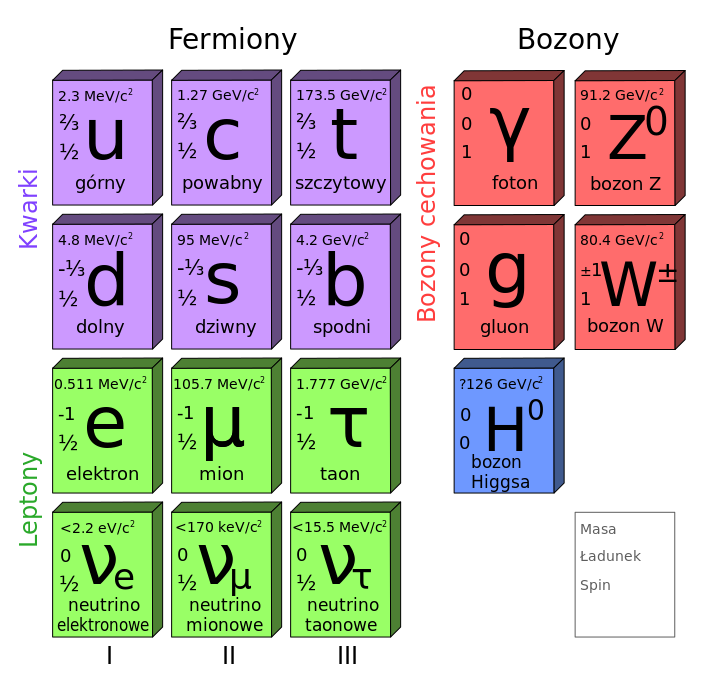
\includegraphics[width=0.7\linewidth]{generalIssues/Figures/standard_model.png}
	\end{subfigure}
	\caption{Cząstki elementarne według Modelu Standardowego.}
	\label{standard_model}
\end{figure}

Fermiony są podstawowymi elementami budującymi materię. Materię trwałą, która nas otacza, tworzą następujące cząstki: elektron, kwark górny (u) oraz kwark dolny (d) np.  dwa kwarki górne i jeden dolny (uud) tworzą proton. Kwarki mają kolor i zapach (są to nazwy nadane umownie pewnym liczbom kwantowym). Do tej grupy cząstek należy też neutrino elektronowe, a grupa ta tworzy pierwszą generację. Kolejne dwie generacje zawieraja po cztery cząstki odpowiadające cząstkom z pierwszej generacji (lecz o różnej masie).

Bozony cechowania przenoszą oddziaływania:
\begin{itemize}
	\item elektromagnetyczne - przenoszone jest przez foton. Oddziaływanie to odbywa się poprzez wytworzenie lub pochłonięcie fotonu.
	\item słabe - powodujące między innymi rozpady beta, przenoszone jest przez bozony $ W^+ $ i $ W^- $ oraz $ Z^0 $.
	\item silne - łączące kwarki w hadrony, przenoszone jest przez osiem rodzajów gluonów, sposób oddziaływania (rodzaj gluonu) oznaczany jest właściwością nazywaną kolorem gluonu. Hadrony złożone są z kwarków występujących przeważnie trójkami (trzy kwarki lub trzy antykwarki tworzą bariony - spin połówkowy, liczba barionowa = 1) lub parami (pary kwark i antykwark tworzą mezony - spin całkowity, liczba barionowa = 0). Właściwością hadronów jest również ich całkowity ładunek elektryczny.
\end{itemize}

Bozon Higgsa (istnienie którego udało się potwierdzić doświadczalnie w 2012 roku) oddziałując z innymi cząstkami nadaje im masę (głównie dotyczy nadawania masy elektronowi, nie dotyczy nadawania masy protonowi i neutronowi, których masa wynika z innego mechanizmu).

Model standardowy jest potwierdzony doświadczalnie, lecz nie jest w pełni satysfakcjonujący z teoretycznego punktu widzenia:

\begin{itemize}
	\item Ma 19 swobodnych parametrów (np. masy cząstek), które należy wyznaczyć doświadczalnie, gdyż teoria nie wyjaśnia ich wartości.
	\item Obliczenia masy Wszechświata nie zgadzają się z obserwowaną ilością materii we Wszechświecie, brakującą materię nazywa się ciemną materią.
	\item W podstawowej wersji nie uwzględnia mas neutrin.
\end{itemize}

Protony i neutrony związane oddziaływaniem silnym (za pośrednictwem mezonów $ \mu $) tworzą jądra atomowe. Protony odpychają się elektrostatycznie, jednak jądro utrzymywane jest w całości przez oddziaływanie silne. Działa ono tylko na niewielką odległość, dlatego jądra zbyt duże i masywne stają się nietrwałe, co prowadzi do samorzutnego ich rozpadu. Liczba protonów w jądrze atomowym to liczba atomowa, a suma liczb protonów i neutronów to liczba masowa.

Obiekt fizyczny złożony z jądra atomowego i znajdujących się w otoczeniu jądra, związanych z nim oddziaływaniem elektromagnetycznym (siłą elektrostatyczną), elektronów to atom. 

Atomy mogą łączyć się w cząsteczki, których względną trwałość zapewniają wiązania chemiczne.

Atomy mogą łączyć się w cząsteczki, których względną trwałość zapewniają wiązania chemiczne. Wiązania chemiczne powstają dzięki wymianie elektronów między atomami, która może odbywać się na dwa sposoby:
\begin{itemize}
	\item kowalencyjny – polegający na uwspólnianiu par elektronów przez dwa lub więcej atomów,
	\item jonowy – polegający na trwałym przeniesieniu elektronów z jednego atomu na drugi, w którego wyniku na jednym z atomów tworzy się całkowity ładunek ujemny, a na drugim dodatni; w efekcie powstaje para jonowa, która jest związana z sobą zwykłymi oddziaływaniami elektrostatycznymi.
\end{itemize}
	
	\subsection{Dualizm korpuskularno-falowy i jego eksperymentalne potwierdzenie.}
	\underline{Dualizm korpuskularno-falowy} – cecha obiektów kwantowych (np. fotonów czy elektronów) polegająca na przejawianiu, w zależności od sytuacji, właściwości falowych (dyfrakcja, interferencja) lub korpuskularnych (dobrze określona lokalizacja, pęd).

Zgodnie z mechaniką kwantową cała materia charakteryzuje się takim dualizmem, chociaż uwidacznia się on bezpośrednio tylko w bardzo subtelnych eksperymentach wykonywanych na atomach, fotonach, czy innych obiektach kwantowych.

Dualizm korpuskularno-falowy jest ściśle związany z falami de Broglie’a – koncepcją, która przyczyniła się do powstania mechaniki kwantowej, a w szczególności do wyprowadzenia równania Schrödingera: $ \lambda = \frac{h}{p} $, gdzie gdzie $ h $ jest stałą Plancka, łączącą wielkości falowe (długość fali $ \lambda $) z korpuskularnymi (pęd $ p $).

Dokonując pomiaru położenia cząstki zawsze znajdujemy ją w przybliżeniu w konkretnym miejscu w przestrzeni (rejestruje ją konkretny detektor). W przypadku \underline{eksperymentów z podwójną szczeliną} uzyskuje się interferencję bądź nie w zależności od tego czy obiekt przejawia właściwości falowe czy cząsteczkowe. Właściwości cząsteczkowe są obserwowane, gdy w szczelinach będzie umieszczony detektor, wykrywający przez którą szczelinę się poruszał obiekt. Przyczyną tego jest istnienie splątania kwantowego i dostępność informacji o obserwablach. Po detekcji cząstki nieoznaczoność jej pędu stopniowo wzrasta, przez co maleje widoczność prążków interferencyjnych.

Young w 1801 r. pierwszy eksperyment przeprowadził ze światłem. Następnie przeprowadzano eksperymenty z elektronami, atomami oraz cząsteczkami. Największe układy, dla których zaobserwowano dualizm korpuskularno-falowy miały 58 (ftalocyjanina), 114 atomów (pochodna ftalocjaniny) i nawet po kilkaset atomów.


	
	\subsection{Hamiltonian w mechanice klasycznej i kwantowej.}
	\underline{Hamiltonian (funkcja Hamiltona)} – funkcja współrzędnych uogólnionych i pędów uogólnionych, opisująca układ fizyczny:\newline
$ H = H(q_1,...,q_N,p_1,...,p_N,t) $, gdzie:\newline
$ q_j $ - współrzędne uogólnione,\newline
$ p_j $ - pędy uogólnione,\newline
$ N $ - liczba stopni swobody,\newline
$ t $ - czas.

Funkcję Hamiltona otrzymuje się z wyrażenia na energię całkowitą układu (przy czym prędkości wyraża się za pomocą pędów) np:

\begin{itemize}
	\item Hamiltonian punktu materialnego poruszającego się z prędkością nierelatywistyczną w potencjale V:\newline
	$ H(t,\textbf{q},\textbf{p}) = \dfrac{\textbf{p}^2}{2m} + V(\textbf{q}) $
	\item Hamiltonian oscylatora harmonicznego poruszającego się w kierunku $ x $:\newline
	$ H(x, p) = \dfrac{p^2}{2m} + \dfrac{m\omega_0^2x^2}{2} $
\end{itemize}

Funkcję Hamiltona można też otrzymać z funkcji Lagrange’a (za pomocą tzw. transformacji Legendre’a). Funkcja Lagrange'a:\newline
$ L(q_1(t),...q_n(t),\dot{q}_1(t),...,\dot{q}_N(t),t) = \\ T(q_1(t),...q_n(t),\dot{q}_1(t),...,\dot{q}_N(t),t) - U(q_1(t),...q_n(t),\dot{q}_1(t),...,\dot{q}_N(t),t) $, gdzie:\newline
$ T $ - energia kinetyczna,\newline
$ U $ - uogólniona energia potencjalna.\newline
$ q_j $ - współrzędna uogólniona,\newline
$ {q}_j $ - prędkość uogólniona.\newline

Dla każdej prędkości uogólnionej $ \dot{q}_j $ wyznacza się odpowiadający jej pęd uogólniony $ p_j $, zdefiniowany jako pochodna funkcji Lagrange’a po prędkości uogólnionej $ \dot{q}_j $:\newline
$ p_j = \dfrac{\partial L}{\partial \dot{q}_j} $

Hamiltonian można znaleźć teraz z funkcji Lagrange’a za pomocą tzw. transformacji Legendre’a:\newline
$ H = H(q_1,...,q_N,p_1,...,p_N,t) = \sum_{i}\dot{q}_j p_j - L(q_1(t),...q_n(t),\dot{q}_1(t),...,\dot{q}_N(t),t)  $ \newline
przy czym konieczne jest wyrażenie prędkości uogólnionych występujących w funkcji Lagrange’a przez pędy uogólnione, gdyż funkcja Hamiltona musi być zapisana jako funkcja pędów uogólnionych. Nie dla wszystkich układów taka transformacja jest możliwa. W przypadku współrzędnych kartezjańskich pędy uogólnione są zwykłymi pędami. We współrzędnych walcowych jako jedną ze współrzędnych uogólnionych cząstki przyjmuje się kąt; wtedy prędkość uogólniona jest prędkością kątową, a pęd uogólniony – obliczany jako pochodna funkcji Lagrange’a po prędkości kątowej – okazuje się być momentem pędu cząstki. W ogólnym przypadku pędy uogólnione mogą nie posiadać prostej interpretacji fizycznej, co wynika z dowolności wyboru współrzędnych uogólnionych.

\underline{Operator Hamiltona} $ \hat{H} $ - operator definiowany w mechanice kwantowej, będący odpowiednikiem funkcji Hamiltona $ H $ (hamiltonianu) mechaniki klasycznej. Operator Hamiltona działa na wektory stanu układu kwantowego: \newline
$ \hat{H}|\Psi(t) \rangle = i\hbar\dfrac{\partial}{\partial t}|\Psi(t) \rangle $\newline
tworząc zależne od czasu równanie Schrodingera. Operator Hamiltona jest jedną z obserwabli, jakie wprowadza mechanika kwantowa, czyli operatorem takim, że jego wartości własne są wielkościami, które można otrzymać w eksperymencie. Wartości własne operatora Hamiltona przedstawiają wartości energii, jakie układ kwantowy może posiadać. Ponieważ energie wyraża się za pomocą liczb rzeczywistych, to implikuje, że operator Hamiltona musi być operatorem hermitowskim (operatorem samosprzężonym) $ \hat{H} = \hat{H}^\dag $. Jest tak dlatego, że tylko operator hermitowski ma wartości własne będące zawsze liczbami rzeczywistymi.

Aby uzyskać postać operatora Hamiltona dla danego układu, w klasycznej funkcji Hamiltona zamienia się współrzędne uogólnione i pędy na odpowiadające im operatory. Najprościej dokonuje się tego, gdy współrzędnymi uogólnionymi są współrzędne kartezjańskie $ x_i $, które pozostawia się bez zmian, a np. w przypadku cząstki swobodnej pędom przypisuje się operatory różniczkowania po sprzężonych z nimi współrzędnych:\newline
$ p_i \rightarrow \hat{p}_i = -i\hbar \frac{\partial}{\partial x_i} $\newline
Operator hamiltona dla cząstki swobodnej w polu $ V(x,t) $ będzie miał więc postać:\newline
$ H(x, p_x, t) = \dfrac{\hat{p}_x^2}{2m} + V(x,t) = \dfrac{-\hbar^2}{2m}\dfrac{\partial^2}{\partial x^2} + V(x,t) $\newline

Jeżeli klasyczna funkcja Hamiltona opisująca dany układ jest niezależna od czasu, to także operator Hamiltona $ \hat{H} $ nie zależy od czasu. Wtedy zamiast ogólnego równania Schrödingera wystarczy rozwiązać równania Schrödingera niezależne od czasu, które jest równaniem własnym hamiltonianu:\newline
$ \hat{H}|\psi_E\rangle = E|\psi_E\rangle $, gdzie:\newline
$ E $ -  wartości własne operatora Hamiltona - wartości te są wartościami energii, jakie układ może posiadać,\newline
$ |\psi_E\rangle $ - stany własne operatora Hamiltona o energiach $ E $.



	
	\subsection{Równanie Schrödingera zależne i niezależne od czasu.}
	\underline{Równanie Schrödingera} – jedno z podstawowych równań nierelatywistycznej mechaniki kwantowej opisujące funkcję falową albo stan układu kwantowego.

Najbardziej ogólna forma zależnego od czasu równania Schrödingera:\newline
$ i\hbar\dfrac{d}{dt}|\Psi(t) \rangle = \hat{H}|\Psi(t) \rangle $, gdzie:\newline
$ i $ - jednostka urojona, \newline
$ \hbar = h/2\pi $, $ h $ - stała Plancka, \newline
$ \hat{H} $ - operator Hamiltona, \newline
$ |\Psi(t) \rangle $ - wektor stanu układu.

Aby rozwiązać równanie Schrödingera dla danego układu kwantowego, należy znaleźć właściwą postać operatora Hamiltona oraz wyrazić wektor stanu w odpowiedniej reprezentacji, np. dla pojedynczej cząstki w jednym wymiarze $ x $, w potencjale $ V(x) $ hamiltonian wygląda następująco:\newline
$ \hat{H} = \dfrac{\hat{p}^2}{2m} + V(x) = \dfrac{\hbar^2}{2m}\dfrac{d^2}{dx^2} + V(x) $

Gdy potencjał nie zależy od czasu, funkcję falową możemy zapisać jako iloczyn części przestrzennej i czasowej:\newline
$ \Psi(x,t) = \psi(x)\psi(t) $ otrzymując następującą formę równania Schrödingera:\newline
$ i\hbar\dfrac{ d(\psi(x)\psi(t))}{dt} = \dfrac{\hbar^2}{2m}\dfrac{d^2(\psi(x)\psi(t))}{dx^2} + V(x)\psi(x)\psi(t) $, następnie odseparowywujemy zmienne i wiedząc, że lewa strona jest tylko zależna od czasu, a prawa tylko od położenia są one równe stałej (na podstawie prawej storny równania stwierdzamy, że stała ta ma wymiar energii):\newline
$ i\hbar\dfrac{1}{\psi(t)}\dfrac{ d\psi(t)}{dt} = \dfrac{1}{\psi(x)}\Big[\dfrac{\hbar^2}{2m}\dfrac{d^2}{dx^2} + V(x)\Big]\psi(x) = E $\newline
Z powyższego równania otrzymujemy dwie zależności:\newline
$ \Psi(x,t) = \psi(x)e^{-iEt/\hbar} $ -  całkowita funkcja falowa różni się od części przestrzennej tylko czynnikiem fazowym,\newline
$ \dfrac{\hbar^2}{2m}\dfrac{d^2\psi(x)}{dx^2} + V(x)\psi(x) = E\psi(x) $ - niezależne od czasu równanie Schrödingera dla przypadku jednowymiarowego cząstki w potencjale $ V(x) $. 

Funkcje $ \psi(x) $ spełniające powyższe równanie przy zadanym potencjale $ V(x) $ nazywamy funkcjami
własnymi, a wartości energii, dla których istnieją te rozwiązania, nazywamy wartościami własnymi.

Funkcja własna jak i jej pochodna musi być skończona, jednoznaczna i ciągła. Gęstość prawodopodobieństwa znaleznia cząstki opisuje wzór:\newline
$ P(x,t) = \Psi^*(x,t)\Psi(x,t) = \psi^*(x)\psi(x) = P(x) $, \newline
Warunek normalizacji dla gęstości prawdopodobieństwa:\newline
$ \int_{-\infty}^{\infty}\Psi^*(x,t)\Psi(x,t) = 1 $

Równanie Schrödingera jest równaniem liniowym, co oznacza, że jeśli $ \Psi_1(x,t) $, $ \Psi_2(x,t) $ są rozwiązaniami tego równania, to również liniowa kombinacja tych funkcji jest rozwiązaniem tego
równania. Uogólniając:\newline
$ \Psi(x,t) = \sum_N a_N\Psi_N(x,t) $ jest rozwiązaniem równania Schrödingera przy dowolnych $ a_N $ gdy $ \Psi_1 $,...,$ \Psi_N $ są rozwiązaniami
tego równania.

	
	\subsection{Podstawy formalizmu kwantowego – wielkości fizyczne, stany, operatory.}
	Stan układu kwantowego reprezentowany jest przez wektor stanu w przestrzeni Hilberta (przestrzeń wektorowa nad ciałem liczb zespolonych). Do oznaczania wektorów stanu stosuje się notację Diraca. Wektor stanu oznacza się przez ket $ |\Psi \rangle $, a wektor dualny (sprzężony) do niego przez $ \langle \Psi | $.

Każda wielkość fizyczna (obserwabla) reprezentowana jest przez hermitowski (lub samosprzężony) operator liniowy działający w przestrzeni stanów (przestrzeni Hilberta). Zbiór wartości własnych tego operatora, nazywany widmem punktowym operatora, interpretuje się jako zbiór możliwych wartości obserwowalnych (pomiarowych). Dla hermitowskich operatorów wartości w widmie są liczbami rzeczywistymi. Stany własne (wektory w łasne) tego operatora do tych wartości własnych interpretuje się jako możliwe stany, w których znajdzie się układ po dokonaniu pomiaru. 

Wektor stanu można zapisać w postaci poniższej sumy:\newline
$ |\Psi\rangle = \sum_i |i \rangle \langle i | \Psi \rangle $

Prawdopodobieństwa otrzymania poszczególnych wartości pomiarów:\newline
$ P_i = |\langle i | \Psi \rangle |^2 $


Operator pędu w reprezentacji położeniowej można otrzymać, używając rozwiązania fali płaskiej do równania Schrödingera pojedynczej cząstki: \newline
$ \Psi(x,t) = e^{\frac{i}{\hbar}(px-Et)} $, gdzie: \newline
$ p $ - pęd cząstki w kierunku $ x $,\newline
$ E $ - energia cząstki.\newline
Pochodna cząstkowa 1-go rzędu wzdłuż $ x $ wynosi:\newline
$ \dfrac{\partial \Psi(x,t)}{\partial x} = \dfrac{ip}{\hbar} e^{\frac{i}{\hbar}(px-Et)} $, stąd:\newline
$ \hat{p} = -i\hbar \dfrac{\partial}{\partial x} $

Ważną cechą kwantowego operatora położenia jest to, że nie komutuje on z operatorem pędu (są to operatory kanonicznie sprzężone). Operatory te spełniają relację komutacyjną:\newline
$ [x_i, p_j] = i\hbar \delta_{ij} $, gdzie:\newline
$ [\textbf{A}, \textbf{B}] = \textbf{A} \textbf{B} - \textbf{B} \textbf{A} $\newline
Powyższa zależność jest matematycznym zapisem zasady nieoznaczoności, która można zapisać również jako:\newline
$ \Delta x \Delta p_x \geq \dfrac{\hbar}{2} $, gdzie:\newline
$ \Delta x, \Delta p_x $ - niepewności wynikające z istoty samego pomiaru (wpływu pomiaru na obiekt mierzony)

	
	\subsection{Kwantowy opis atomu wodoru. Liczby kwantowe.}
	Energię potencjalną będącą wynikiem oddziaływania kulombowskiego pomiędzy pojedynczym elektronem i protonem w atomie wodoru opisuje poniższy wzór:\newline
$ U(r) = \dfrac{e^2}{4\pi \epsilon_0 r} $, gdzie:\newline
$ r $ - odległość elektronu od protonu.\newline
Energia potencjalna jest funkcją odległości r od jądra. Jest to pole centralne.

\begin{figure} [H]
	\centering
	\begin{subfigure}{.99\textwidth}
		\centering
		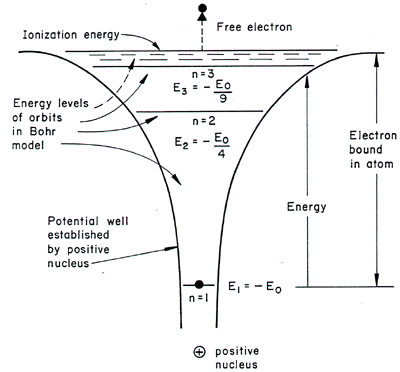
\includegraphics[width=1.0\linewidth]{generalIssues/Figures/potential.png}
	\end{subfigure}
	\caption{Energia potencjalna oddziaływania kulombowskiego pomiędzy elektronem, a jądrem w atomie wodoru.}
	\label{maxwell}
\end{figure}

Równanie Schrodingera dla takiego potencjału ma postać:\newline
$ -\dfrac{\hbar}{2m_e} \nabla^2 \Psi(\vec{r}) = (E-U(\vec{r})) \Psi(\vec{r}) $\newline

Równanie to można rozwiązać przechodząc do układu współrzędnych sferycznych, a następnie sprowadzając je do układu równań jednowymiarowych stosując separację zmiennych:\newline
$ \Psi(\vec{r}) = R(r)\Theta(\theta)\phi(\varphi) $\newline
Rozwiązanie dla funkcji $ \phi(\varphi) $:\newline
$ \phi(\varphi) = e^{im_l \varphi} $ implikuje:\newline
$ e^{im_l 0} = e^{im_l 2\pi} $, warunek ten jest spełniony gdy:\newline
$ |m_l| = 0, 1, 2, 3 ... $.

Liczba kwantowa $ m_l $, nazywana magnetyczną liczbą kwantową,jest związana z orientacją w przestrzeni wektora momentu pędu. Jeżeli atom znajduje się w zewnętrznym polu magnetycznym, to jego energia zależy od tej liczby kwantowej. Liczba kwantowa $ m_l $ może być tylko liczbą całkowitą. 

Rozwiązanie dla funkcji $ \Theta(\theta) $ implikuje istnienie liczby kwantowej $ l = |m_l|, |m_l|+1, |m_l|+2 ... $ nazywanej orbitalną liczbą kwantową, będącą miarą wielkości momentu pędu związanego ze stanem kwantowym: \newline
$ L = \hbar \sqrt{l(l+1)} $ - orbitralny moment pędu.\newline
$ L_z = \hbar m_l $ - rzut wektora momentu pęduna oś OZ.\newline
Obie powyższe wielkości są skwantowane.

Dostępne stany energii opisuje równanie:\newline
$ E = -\dfrac{1}{2} m_e c^2 (Z\alpha)^2 \dfrac{1}{n_r + l + 1} $, gdzie:\newline
$ Z $ - liczba atomowa (dla wodoru $ Z $ = 1),\newline
$ \alpha \approx 1/137 $ - stała struktury subtelnej,\newline
$ n_l = 0, 1, 2 ... $ - radialna liczba kwantowa,\newline
$ n = n_r + l + 1 $ - główna liczba kwantowa (jest zawsze całkowitą liczbą dodatnią).

Jest to dokładnie ten sam wzór, który wynika z modelu Bohra dla energii dozwolonych stanów związanych.

Np. dla energii $ E_0 = E(n = 1) $ mamy tylko jeden możliwy stan ($n = 1, l = 0, m_l = 0$). Energii $ E_1 = E(n = 2) $ odpowiadają cztery zdegenerowane stany:\newline
($n = 2, l = 0, m_l = 0$),\newline
($n = 2, l = 1, m_l = +1$),\newline
($n = 2, l = 1, m_l = 0$),\newline
($n = 2, l = 1, m_l = -1$).
	
    \section{Specjalność: Eksploracja Danych i Modelowanie Interdyscyplinarne}
    
    \subsection{Automaty komórkowe.}
    Automat komórkowy – system składający się z pojedynczych komórek, znajdujących się obok siebie. Ich układ przypomina szachownicę lub planszę do gry.

Każda z komórek może przyjąć jeden ze stanów, przy czym liczba stanów jest skończona, ale dowolnie duża.

Przestrzeń stanów określamy poprzez zdefiniowanie wartości wybranej ze skończonego zbioru $ Q $, który może być podzbiorem zbiorów podstawowych (np. liczb, liter) lub złożonych (struktury, obiekty). 

Poprzez przestrzeń stanów opisane zostają wszystkie możliwe stany komórki. Od dobrego określenia przestrzeni stanów zależy szybkość automatu komórkowego, jak i jego podstawowe cechy charakterystyczne. Stan komórki zależy od aktualnych stanów komórek z otoczenia, jak i komórka swoim stanem wpływa bezpośrednio na stany swoich sąsiadów.

Istnieją trzy konstrukcyjne czynniki automatu komórkowego, które w zasadniczy sposób wpływają na strukturę siatki:
\begin{itemize}
\item wymiar przestrzeni, zależny od wielkości badanego problemu (siatka 1D, 2D, 3D, nD),
\item warunek regularności, mówiący o całkowitym zapełnieniu siatki przez jednakowe komórki (komórki trójkątne, kwadratowe, sześciokątne dla 2D, sześcienne lub w kształcie dwunastościanów rombowych dla 3D etc.),
\item liczba sąsiadów (zależna od obu powyższych, rysunek~\ref{neighbours} przedstawia podstawowe typy sąsiedztwa).
\end{itemize}

\begin{figure} [H]
	\centering
	\begin{subfigure}{.6\textwidth}
		\centering
		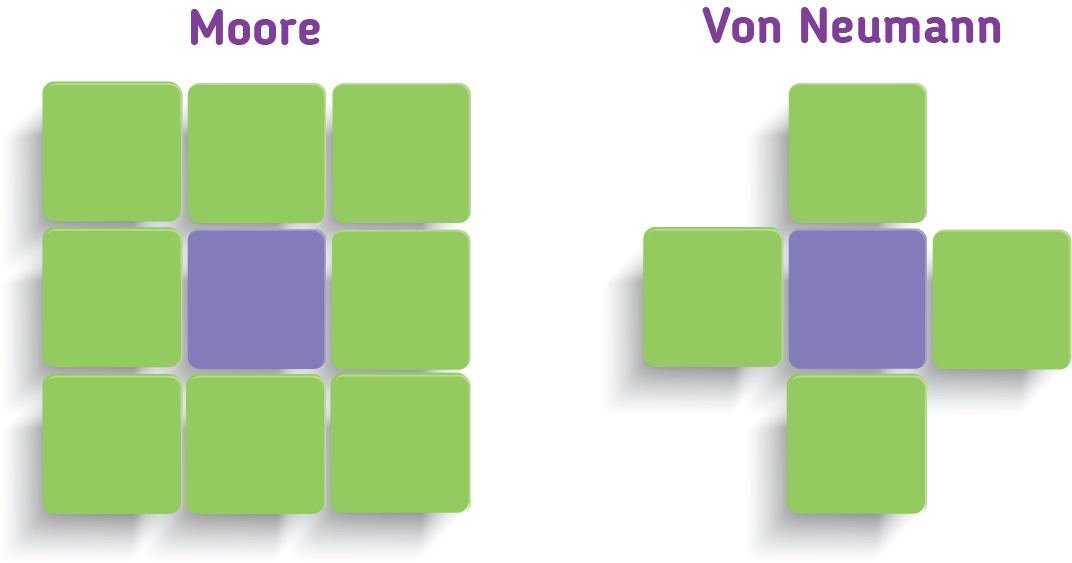
\includegraphics[width=1.0\linewidth]{EDMIIssues/Figures/sasiedztwa.png}
	\end{subfigure}
	\caption{Podstawowe typy sąsiedztwa.}
	\label{neighbours}
\end{figure} 

Budowa wszystkich komórek musi być identyczna (muszą mieć tyle samo sąsiadów, takie same zbiory stanów itp.)

Ważnym elementem konstrukcyjnym automatów komórkowych są warunki początkowe, czyli stany poszczególnych komórek w zerowej iteracji, czyli na samym początku. To od ustawienia początkowego komórek zależy dalsza ewolucja automatu, jego zachowanie, stan końcowy, tym samym powodzenie całej symulacji. Niektóre automaty komórkowe z założenia muszą mieć w odpowiedni sposób ustalone warunki początkowe

Zachowanie automatu jest definiowane m.in. poprzez warunki brzegowe, które moga być np. periodyczne, pochłaniające, czy odbijające.

Stan komórki $ x $ w chwili $ t $ oznaczmy jako $ x_t $, a stan sąsiedztwa jako $ u(x_t) $. Dla takich kryteriów stan komórki $ x $ w kolejnym kroku iteracji można opisać wzorem:\newline
$ x_{t+1} = f(u(x_t), x_t) $, gdzie:\newline
$ f $ - funkcja przejścia, która może być opisana różnego rodzaju zależnościami, np. jako tabela przejść, w postaci algorytmicznej lub jako zbiór reguł.

Po ustaleniu i zdefiniowaniu wszystkich elementów składowych automatu komórkowego można przejść do nakładania reguł na siatkę, czyli aktualizowania jej.

Podział automatów komórkowych według Wolframa:
\begin{itemize}
	\item Klasa I: Automaty niezmienne – ewoluują do czasu, kiedy wszystkie komórki osiągną identyczny stan niezależnie od stanu początkowego (zbieżne).
	\item Klasa II: Automaty ewoluujące do stanu stabilnego lub okresowych wzorców (okresowe).
	\item Klasa III: Automaty wykazujące nieporządek zarówno lokalnie, jak i globalnie, nie wykazujące żadnego wzorca (chaotyczne).
	\item Klasa IV: Automaty wykazujące bardziej złożone, długotrwałe zachowanie („żywe”).
\end{itemize}

Technika automatów komórkowych jest używana do symulacji komputerowych w wielu problemach nauki i techniki. Automaty te dostarczają również wielu zagadnień teorii dynamiki nieliniowej.

Jednym z pierwszych i najbardziej znanych przykładów automatu komórkowego jest \textit{Gra w życie} (\textit{Life}, \textit{The game of life}). Reguły tego automatu według Conwaya:
\begin{itemize}
	\item Martwa komórka, która ma dokładnie 3 żywych sąsiadów, staje się żywa w następnej jednostce czasu (rodzi się),
	\item Żywa komórka z 2 albo 3 żywymi sąsiadami pozostaje nadal żywa; przy innej liczbie sąsiadów umiera (z „samotności” albo „zatłoczenia”).
\end{itemize}

    
    \subsection{Podstawowe twierdzenie algorytmów genetycznych.}
    \underline{Algorytmy genetyczne} stanowią podgrupę algorytmów ewolucyjnych. Są to algorytmy poszukiwania oparte na mechanizmach doboru naturalnego oraz dziedziczności. Oznacza to, iż wykorzystujemy ewolucję aby poprzez operatory (mutacje i krzyżowanie) otrzymać z niemal losowych danych to co będziemy uważać za poprawne. AG pracują na zakodowanej formie rozwiązań oraz na całej populacji rozwiązań. Bazują tylko na funkcji celu (nie musi być ona ciągła ani różniczkowalna, ani także być funkcją analityczną).

\underline{Schematem $ H $} nazywamy wzorzec opisujący podzbiór ciągów podobnych ze względu na ustalone pozycje. Alfabet składający się z $ k $ symboli i ciągów $ l $ elementowych posiada $ k^l $ ciągów i $ (k+1)^l $ schematów. Np. dla alfabetu dwuelementowego $ \{0, 1\} $ alfabet schematu $ V^+ = \{0, 1, *\} $, gdzie $ * $ - oznacza pozycję nieustaloną.

\underline{Rząd schematu} to liczba ustalonych pozycji we wzorcu o(H) np:\newline
$ o(\{01**01**\}) = 4 $

\underline{Rozpiętość schematu} to odległość między dwiema skrajnymi ustalonymi pozycjami $ \delta (H) $ np:\newline
$ \delta(\{01**01**\}) = 5 $

$ m(H, t) $ to \underline{liczba reprezentantów} schematu $ H $, czyli jak dużo osobników populacji pasuje do schematu $ H $ w czasie $ t $.

\underline{Wartość oczekiwana} liczby reprezentantów schematu $ H $ w następnym pokoleniu:\newline
$ E(m(H, t+1)) = m(H, t)\cdot n \cdot \dfrac{f(H)}{\sum_i f_i} = m(H, t) \cdot \dfrac{f(H)}{\overline{f}} $, gdzie:\newline
$ f(H) $ - współczynnik dostosowania schematu $ H $,\newline
$ \overline{f} = \dfrac{\sum_i f_i}{n} $ - średni współczynnik dostosowania całej populacji.

\underline{Prawdopodobieństwo przeżycia schematu}:\newline
$ p_s(H) \geq \dfrac{\delta (H)}{l-1} $

Oczekiwana liczba reprezentantów schematu H w następnym pokoleniu, otrzymanym w wyniku reprodukcji, krzyżowania i mutacji, spełnia następującą nierówność:\newline
$ m(H, t+1) \geq m(H, t) \cdot \dfrac{f(H)}{\overline{f}} [1 - p_c \dfrac{\delta (H)}{l-1} - p_m o(H)] $, gdzie: \newline
$ p_c $ - prawdopodobieństwo krzyżowania,\newline
$ p_m $ - prawdopodobieństwo mutacji.

Dla schematów niskiego rzędu i o małej rozpiętości  destruktywne efekty krzyżowania i mutacji można pominąć, a wtedy:\newline
$ m(H, t+1) = m(H, t) \cdot (1+ \epsilon ) $, przy założeniu, że $ f(H, t) = (1+ \epsilon )\overline{f} $ czyli schemat $ H $ ma dopasowanie o $ \epsilon $ większe niż średnia z populacji. Zakładając że $ \epsilon $ nie zmienia się w czasie, wówczas długoterminowy efekt przetwarzania schematu $ H $ będzie następujący:\newline
$ m(H, t+s) = m(H, t)(1 + \epsilon)^s $ - oceniane "powyżej średniej" schematy o "niskiego rzędu" i o "małej rozpiętości" uzyskują wykładniczo rosnącą liczbę reprezentantów w kolejnych pokoleniach. Ta konkluzja jest nazywana \underline{podstawowym twierdzeniem algorytmów genetycznych}.
    
    \subsection{Sieci bezskalowe.}
    \underline{Sieć bezskalowa} to sieć o potęgowym rozkładzie liczby połączeń między węzłami:\newline
$ P(k) = \dfrac{C}{k^{\gamma}} $, gdzie:\newline
$ k $ - liczba węzłów, \newline
$ \gamma $ - parametr właściwy dla danej sieci i zwykle przyjmującym wartości z zakresu $ (2, 3) $.

Potęgowy rozkład stopni wierzchołków jest cechą charakterystyczną wielu sieci rzeczywistych (np. sieć energetyczna, sieć www). Rozkład potęgowy nie ma naturalnej skali, jest bezskalowy. Oznacza to, że mówienie o średnich wartościach stopni wierzchołków w takich sieciach jest co najmniej niewskazane, a wielu wypadkach posługiwanie się ideą średniego stopnia prowadzi do poważnych błędów. W sieci o potęgowym rozkładzie stopni wierzchołków wiele węzłów ma tylko jedną krawędź (tłusty ogon), ale można też znaleźć węzły z ogromną liczbą krawędzi, tzw. huby.

Nie wszystkie tłustoogoniaste rozkłady są potęgowe. Zlogarytmizujmy obie strony równania opsiującego rozkład potęgowy:\newline
$ ln(P(k)) = -\gamma ln(k) + ln(C) $\newline
Rozkład potęgowy charakteryzuje się tym, że przedstawiony w nowych współrzędnych tj. $ X = ln(k) $, $ Y = ln(P(k)) $ staje się równoważny liniowej zależności $ Y = aX + b $.

Sieci bezskalowe charakteryzują się łatwością w niszczeniu topologii sieci, poprzez usunięcie wierzchołków o dużej liczbie połączeń tzw. "hub-ów", które są krytyczne dla łączności sieci np. awaria istotnego węzła sieci energetycznej, albo atak hakerski na ruchliwy serwer.

Sieci bezskalowe mogą być generowane zgodnie z modelem Barabasi-Alberta. Proces konstrukcji takiej sieci wygląda następująco:
\begin{itemize}
	\item Rozpocznij proces od pewnego niewielkiego zbioru wierzchołków (zazwyczaj jednego).
	\item W każdym kroku dodaj jeden wierzchołek i dołącz do już istniejących dając preferencje tym którzy już mają dobrą łączność (prawdopodobieństwo dodania krawędzi do wierzchołka $ v $jest proporcjonalne do aktualnego stopnia $ d_v $ - wiązanie preferencyjne). Ilość dodawanych w każdym kroku krawędzi jest parametrem modelu $ m $.
\end{itemize}

Powstałe w ten sposób sieci charakteryzują się rozkładem krawędzi:\newline 
$ P(k) \approx \dfrac{2m^2}{k^3} $.

Prawo potęgowe wraz z wykładnikiem są niezmiennicze dla losowego podgrafu (z dużym prawdopodobieństwem). Tutaj pojawia się wyjaśnienie terminu ”bezskalowy”.

\underline{Sieci małych światów:}\newline \textit{W eksperymencie przeprowadzonym w 1967 roku amerykański socjolog Stanley Milgram wysłał do przypadkowo wybranych ludzi 160 listów zawierających wyjaśnienie eksperymentu, zdjęcie, nazwisko i adres pewnej osoby oraz instrukcję postępowania. Jeżeli adresat znał osobiście człowieka wymienionego w liście, miał przesłać list bezpośrednio do niego. W przeciwnym wypadku list powinien zostać przesłany do innego znajomego, o którym adresat mógł sądzić, że może znać poszukiwaną osobę lub przynajmniej znać kogoś, kto tę osobę zna osobiście. Celem eksperymentu było ustalenie, jak długi jest łańcuch znajomych gwarantujący dostarczenie przesyłki do adresata.  Choć większość listów zaginęła, to jednak te 42, które dotarły do poszukiwanej osoby, dostarczyły zaskakujących wyników. Okazało się, że paru listom wystarczyło zaledwie dwóch pośredników by dotrzeć do celu. W kilku innych przypadkach pośredników było kilkunastu. Jednak, po uśrednieniu wyników, okazało się, że statystyczny list przeszedł przez ręce jedynie sześciu osób. Eksperyment Milgrama dowiódł prawdziwości obiegowego porzekadła (znanego również Barneyowi), że świat jest mały. Mimo że sieć społeczna liczy kilka miliardów ludzi, to średnia droga między dowolną parą węzłów w takiej sieci wynosi około sześciu. Ponad dwadzieścia lat po eksperymencie Milgrama ukute zostało nawet sformułowanie „sześć uścisków dłoni” albo „sześć stopni separacji”. } Żródło: \newline (\url{http://www.if.pw.edu.pl/~agatka/moodle/charakterystyki.html#x1-2002r1})
	
	\subsection{Agentowe modele dynamiki opinii.}
	\underline{Model wpływu społecznego}\newline
Wprowadźmy następujące oznaczenia:
\begin{itemize}
	\item $ \sigma_i(t) $ - opinia $ i $-tego agenta, $ \sigma_i(t) \in \{-1, 1\} $
	\item $ I_i(t) $ - "pole społeczne" oddziałujące na $ i $-tego agenta (wynika ono z obecności innych agentów)
	\item $ S_i $ - możliwość popierania (podtrzymania opinii) i-tego agenta, $ S_i $ > 0
	\item $ \prod_i $ - umiejętność perwazji (przekonania do swojej opinii) $ i $-tego agenta, $ \prod_i $ > 0
	\item $ d_{ij} $ - odległość społeczna między $ i $-tym, a $ j $-tym agentem
	\item $ g(d_{ij}) $ - osłabienie oddziaływań pomiędzy agentami w zależności od ich odległości społecznej, zazwyczaj $ g(d_{ij}) = A \cdot d_{ij}^{\alpha} $, $A, \alpha > 0 $, $ g(d_{ij}) = g(0) = \dfrac{1}{\beta} $
	\item $ \beta $ - parametr przekonania do własnej opinii
\end{itemize}

Poniższy wzór opisuje dynamikę modelu:\newline
$ \sigma_i(t + \Delta t) = - sign[\sigma_i (t) I_i(t)] $, gdzie:\newline

$ I_i(t) = \sum_j \dfrac{-[\sigma_i(t)\sigma_j(t) + 1]S_j}{2g(d_{ij})} + \sum_j \dfrac{[\sigma_i(t)\sigma_j(t) - 1]\prod_j}{2g(d_{ij})} + \eta_i(t) $, gdzie:\newline

$ \eta_i(t) $ – czynnik temperaturowy (szum losowy) o właściwościach $ <\eta_i(t)> = 0 $,  $ <(\eta_i(t))^2> = T $.
Kiedy stworzymy dwie sieci (grupy) agentów, o różnych opiniach, w których $ T_1 > T_2 $ i porównamy je ze sobą to grupa o wyższej temperaturze jest bardziej podatna na zmianę opinii.

Wybrany agent zmieni swoja opinię na przeciwną, kiedy pole społeczne
przyjmie wartość dodatnią. Innymi słowy, jego opinia ulegnie zmianie, wtedy gdy presja otoczenia będzie wystarczająco duża.

\underline{Model silnego lidera}\newline
Zakładamy poniższe wartości parametrów:\newline
$ \forall i \neq L, S_i = \prod_i = 1, S_L = \prod_L \gg 1 $

Otrzymujemy poniższe równanie na "pole społeczne":\newline
$ I_i(t) = \sum_{i\neq L} \dfrac{-\sigma_i(t)\sigma_j(t)}{g(d_{ij})} - \dfrac{\sigma_i(t)\sigma_L(t)}{g(d_{iL})}S_L $

\begin{figure} [H]
	\centering
	\begin{subfigure}{.99\textwidth}
		\centering
		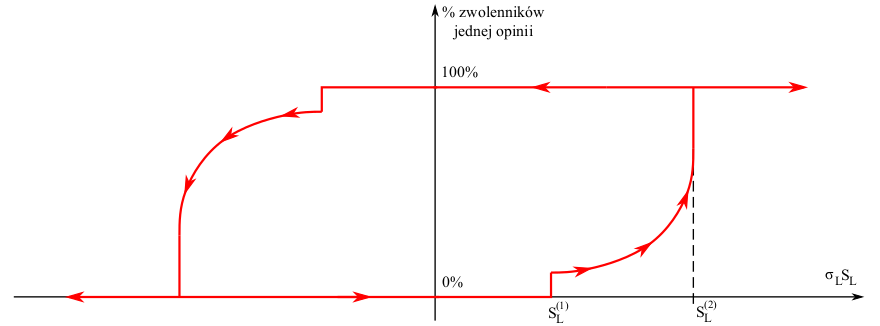
\includegraphics[width=1.0\linewidth]{EDMIIssues/Figures/lider.png}
	\end{subfigure}
	\caption{Proces zwolenników jednej opinii w funkcji iloczynu siły perswazji lidera i jego opinii. Wykres ten przypomina pętle histerezy, obserwowaną m.in. w zjawiskach magnetycznych.}
	\label{lider}
\end{figure}

Dla modelu silnego lidera istnieje wartość krytyczna $ S_L $ po której wszyscy agenci w grupie przyjmują wspólną opinię (rys.~\ref{lider}).

\underline{Model votera (wyborcy)} - agenci umiejscowieni są w sieci, w której możemy wyróżnić najbliższe sąsiędztwo każdego z nich. Każdy agent posiada pewną opinię (stan) $ s_i(t) \in {-1, 1} $. Dynamika przebiega w sposób następujący sposób:
\begin{itemize}
	\item Wylosuj agenta $ i $,
	\item Wylosuj agenta $ j $ będącego sąsiadem agenta $ i $,
	\item Agent $ i $ przyjmuję opinię agenta $ j $: $ s_i(t+\Delta t) = s_j(t) $.
\end{itemize}

W przypadku kiedy sieć jest prosta (tzn. każdy agent ma jednakową liczbę sąsiadów) wtedy układ osiąga stan równowagi $ <s_i> = const $. Innymi słowy liczba aktywnych interfejsów $ \rho (t) $ (połączeń agentów o przeciwnych opiniach) zanika w czasie.

Model votera można wzbogacić o koewolucję (ewoluuj ą zarówno stany węzłów jak i topologia samej
sieci). Dynamika koewolucji:
\begin{itemize}
	\item Z prawdopodobieństwem $ 1 - p $ agent $ i $ przyjmuje stan agenta $ j $, tak jak w zwykłym modelu votera,
	\item z prawdopodobieństwem $ p $ agent $ i $ zrywa połączenie z agentem $ j $ i nawiązuje połączenie z losowym agentem, który nie jest jego sąsiadem i posiada taką samą opinie.
\end{itemize}

Załóżmy, że po bardzo długim czasie ($ t \to \infty $) średnia liczba linków aktywnych wynosi $ \rho_s = const. $ Istnieje wtedy pewne prawdopodobieństwo krytyczne $ p = p_c $, dla którego $ \rho_s = 0 $ (rys.~\ref{density}).

\begin{figure} [H]
	\centering
	\begin{subfigure}{.7\textwidth}
		\centering
		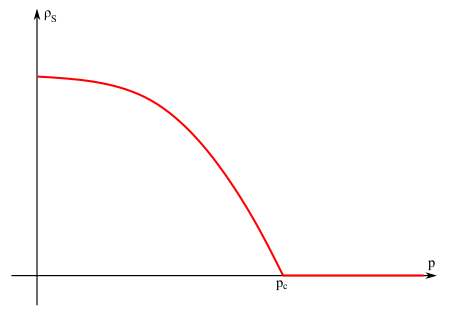
\includegraphics[width=1.0\linewidth]{EDMIIssues/Figures/density.png}
	\end{subfigure}
	\caption{Wykres zależności średniej gęstości aktywnych połączeń po bardzo długim czasie w funkcji prawdopodobieństwa $ p $.}
	\label{density}
\end{figure}

\underline{Model Axelroda} - każdemu agentowi przypisujemy wektor cech (np. wyznawana religia, poglądy polityczne) o długości $ F $, z których każda może posiadać $ q $ wariantów. Przebieg dynamiki:
\begin{itemize}
	\item wybieramy losowo agenta $ i $,
	\item wybieramy losowo agenta $ j $ z najbliższego sąsiedztwa agenta $ i $
	\item obliczamy liczbę wspólnych cech agentów $ i, j$:\newline
	$ l(i, j) = \sum_{f=1}^F \delta_{\sigma_{i,f}\sigma_{j,f}} $, gdzie $ \sigma_{i,f} $ - wariant cechy $ f $, agenta $ i $
	\item Spośród wszystkich cech, takich, że $ \sigma_{i,f} \neq \sigma_{j,f} $ wybieramy cechę $ k $ i zmieniamy opinię agenta $ i $: $\sigma_{i,k}(t+\Delta t) = \sigma_{j,k}(t) $ z prawdopodobieństwem $ p = \dfrac{l(i,j)}{F} $
\end{itemize}

\underline{Model większościowy} - zawiera $ N $ agentów, z których każdy ma opinię $ \pm 1 $. W dowolnej chwili czasu wybieramy $ m $ połączonych ze sobą agentów (zwykle losuje się jednego agenta oraz jego $ m - 1 $ różnych sąsiadów). Każdy agent z tak wylosowanej grupy przyjmuję opinię większości. Prawdopodobieństwo wylosowania agenta z opinią +1:\newline
$ a(t) = \dfrac{N_a(t)}{N} $, gdzie $ N_a(t) $ - liczba zwolenników opini +1 w chwili $ t $.

W najprostszym przypadku zakładamy, że wszyscy agenci są połączeni oraz $ m = 3 $. Wtedy:\newline
$ N_a(t+\Delta t) = N_a(t) + a(t)^2\cdot [1-a(t)] \cdot (+1) + a(t) \cdot [1-a(t)]^2 \cdot (-1) $,\newline
$ a(t + \Delta t) - a(t) = \dfrac{1}{N}a(t)[1-a(t)][2a(t) - 1] $.\newline
Jeśli za $ \Delta t $ przyjmiemy $ N $ wtedy otrzymamy poniższe równanie różniczkowe:\newline
$ \dot{a} = a(t + \Delta t) - a(t) = a(1-a)(2a - 1) = f(a) $\newline
Punkty stałe (miejsca zerowe funckji $ f(a) $) tego dynamicznego układu:\newline
$ a_- = 0, a_0 = 0.5, a_+ = 1 $
Stabilność otrzymancyh trzech punktów stałych badamy obliczając wykładnik Liapunowa $ \lambda (a) $ równy pochodnej $ f'(a) = -6a^2 +6a - 1 $ w tych punktach: \newline
$ \lambda(a_-) = -1 < 0 $ - punkt stabilny,\newline
$ \lambda(a_+) = -1 < 0 $ - punkt stabilny,\newline
$ \lambda(a_0) = 1/2 > 0 $ - punkt niestabilny.
	
	\subsection{Sieć neuronowa typu Hopfielda.}
	\underline{Sieć Hopfielda} jest przykładem sieci ze sprzężeniem zwrotnym (tzw. sieć rekurencyjna), gdzie wyjścia poszczególnych neuronów są podawane z odpowiednimi wagami na wejścia każdego z neuronów. Oczywiście do każdego neuronu podpięte jest wejście, którym doprowadzana jest odpowiednia składowa wektora testowego. Założenia:
\begin{itemize}
	\item całkowite połącznie neuronów,
	\item neurony 2-stanowe,
	\item symetryczne połączenia synaptyczne
	\item synchroniczna dynamika sieci
\end{itemize}

\begin{figure} [H]
	\centering
	\begin{subfigure}{.69\textwidth}
		\centering
		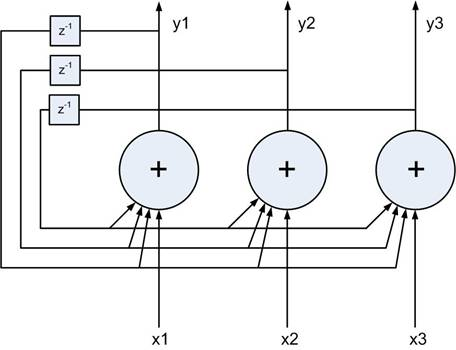
\includegraphics[width=1.0\linewidth]{EDMIIssues/Figures/hopfield.jpg}
	\end{subfigure}
	\caption{Równania Maxwella.}
	\label{hopfield}
\end{figure}

W sieciach Hopfielda waga połączenia wyjścia neuronu z własnym wejściem jest zerowana. Wymagane jest także, aby macierz wag $ W $ była symetryczna.

Funkcja aktywacji pojedynczego neuronu wygląda następująco:\newline
$ y_i(t+1) = 1 $, gdy $ \sum_{j=1}^N w_{ij}y_j(t) + x_i(t) + \xi_i(t) > 0 $,]\newline
$ y_i(t+1) = y_i(t) $, gdy $ \sum_{j=1}^N w_{ij}y_j(t) + x_i(t) + \xi_i(t) = 0 $,\newline
$ y_i(t+1) = -1 $, gdy $ \sum_{j=1}^N w_{ij}y_j(t) + x_i(t) + \xi_i(t) < 0 $, gdzie:\newline
$ i $ oraz $ j $ oznaczają numery neuronów $ N $-neuronowej sieci Hopfielda, $ \xi $ oznacza szum (np. gaussowski o $ \mu $ = 0),  natomiast $ t $ przedstawia chwilę czasową. Należy również zwrócić uwagę na to, że składowe wektora $ x $ w chwili czasowej $ t=0 $ są przepisywane na wyjścia neuronów, natomiast dla $ t>0 $ wejścia są „odpinane” od neuronów ($ x=0 $).

W trybie uczenia, na podstawie zbioru wektorów uczących obliczane są wagi. Najprostszą metodą (wykorzystywaną w naszym przykładzie) uczenia sieci jest reguła Hebb’a. Wagi obliczane są według wzoru:\newline
$ w_{ij} = \dfrac{1}{N} \sum_{k=1}^K x_i^{(k)}x_j^{(k)} $, gdzie $ k $ oznacza numer wektora uczącego, a $ K $ liczbę wszystkich wektorów uczących.

Okazuje się, że gdy na wejście sieci podamy wektor identyczny z wzorcem, wówczas sieć nie zmieni swojego stanu, rozpoznaje ona również obrazy „niewiele” różniące się od wzorców. W niektórych przypadkach pojawia się kolejna cecha sieci Hopfielda - pamiętanie zależności pomiędzy sąsiednimi pikselami, a nie ich wartości. Wtedy otrzymujemy obraz wzorca z odwróconymi kolorami.

Miara podobieństwa wzorca $ k $-tego (pokrycie ang. \textit{overlap}):\newline
$ m^k(t) = \dfrac{1}{N} \sum_{i=1}^{N} y_i(t)x^{(k)}_i $.

Gdy:\newline
$ m^k = 1 $ - całkowita zgodność wzorca,\newline
$ m^k = 0 $ - całkowita niezgodność wzorca,\newline
$ m^k = -1 $ - stan sieci jest negatywem wzorca.

Sieć Hopfielda jest ograniczona ilością wzorców, które może zapamiętać i skutecznie rozróżniać. Jeśli $ p $ - ilość zapamiętanych wzorców, a $ N \to \infty $ - liczba neuronów, to $ p_c = \dfrac{p}{N} \approx 0,138 $, przy założeniu, że średnie pokrycie wzorców nie spada poniżej 95\%.

Liczbę identycznych bitów w dwóch stanach sieci nazywamy odległością Hamminga. Proces ewaluacji wzorca wejściowego zatrzymujemy, gdy wrzozec wyjściowy zbliży się na pewną, ustaloną odległość Hamminga do któregoś z zapamiętanych wzorców.



	
	\subsection{Naiwny klasyfikator Bayesa.}
	\underline{Naiwny klasyfikator Bayesa} - klasyfikator oparty na założeniu o wzajemnej niezależności zmiennych objaśniających (predyktorów). Często nie mają one żadnego związku z rzeczywistością i właśnie z tego powodu nazywa się je naiwnymi. Bardziej opisowe jest określenie – „model cech niezależnych”. Model prawdopodobieństwa można wyprowadzić korzystając z \underline{twierdzenia Bayesa} wiążącego prawdopodobieństwa warunkowe dwóch zdarzeń warunkujących się nawzajem:\newline
$ P(A|B) = \dfrac{{P(B|A)P(A)}}{P(B)} $, gdzie:\newline
$ A $ i $ B $ - zdarzenia,\newline
$ P(A|B) $ - prawdopodobieństwo warunkowe, tj. prawdopodobieństwo zajścia zdarzenia $ A $, o ile zajdzie zdarzenie $ B $.

\underline{Przykład} zastosowania twierdzenia Bayesa:\newline
$ B $ -  zdarzenie "u pacjenta występuje wysoka gorączka" (w badanej populacji $ P(B) = 0.2 $),\newline
$ A $ - zdarzenie "pacjent ma grypę" (w badanej populacji $ P(A) = 0.1 $),\newline
$ P(B|A) = 0.7 $ - na podstawie statystyki populacji wiemy, że jeśli pacjent ma grypę to na 70\% ma gorączkę.\newline
Na podstawie twierdzenia Bayesa możemy obliczyć prawdopodobieństwo, że pacjent mający gorączkę, jest chory na grypę:\newline
$ P(A|B) = \dfrac{{P(B|A)P(A)}}{P(B)} = \dfrac{0,7\cdot 0,1}{0,2} = 0,35$ 

Korzystając z twierdzenia Bayesa:\newline
$ p(C|F_1,...,F_n) = \dfrac{P(C)P(F_1,...,F_n|C)}{P(F_1,...,F_n)} $, gdzie:\newline
$ C $ - klasa zależna od $ n $ opisujących zmiennych niezależnych $ F_i $.

W praktyce interesujący jest tylko licznik ułamka, bo mianownik nie zależy od $ C $. Licznik ułamka jest równoważny do łącznego modelu prawdopodobieństwa:\newline
$ P(C, F_1,...,F_n) $\newline $ = P(C)P(F_1,...,F_n|C) $\newline $ = P(C)P(F_1|C)P(F_2,...,F_n|C, F_1) $\newline $ = P(C)P(F_1|C)P(F_2|C, F_1)P(F_3,...,F_n|C, F_1, F_2) $\newline
$ = P(C)P(F_1|C)P(F_2|C, F_1)P(F_3|C, F_1, F_2)P(F_4,...,F_n|C, F_1, F_2, F_3) $\newline itd...\newline
Włącza się teraz "naiwną" warunkową zależność, zakładając, że każda cecha $ F_i $ jest warunkowo niezależna od każdej innej cechy. Oznacza to, że:\newline
$ p(F_i|C, F_j) = P(F_i|C) $ więc model można wyrazić jako:\newline
$ P(C, F_1,...,F_n) = p(C)p(F_1|C)p(F_2|C)...p(F_n|C) = p(C) \prod_{i=1}^{n} p(F_i|C) $

Oznacza to, że pod powyższymi niezależnymi założeniami, warunkowe rozmieszczenie nad klasą zmiennych $ C $ można zapisać jako: \newline
$ p(C|F_1,...,F_n) = \dfrac{1}{Z} p(C) \prod_{i=1}^{n} p(F_i|C) $, gdzie:\newline
$ Z $ - współczynnik skalowania zależny wyłącznie od zmiennych $ F_1,...,F_n $.

Modele tej formy są łatwiejsze do zrealizowania, gdy rozłoży się je na czynniki zwane klasą „prior” $ p(C) $ i niezależny rozkład prawdopodobieństwa $ p(F_i|C) $. Jeśli są $ k $ klasy i jeśli model dla $ p(F_i) $ może być wyrażony przez r parametrów, wtedy odpowiadający naiwny model Bayesa ma $ (k-1) + nrk $ parametrów. W praktyce często $ k = 2 $ (klasyfikacja binarna) i $ r = 1 $ (zmienna Bernouliego jako cecha), wtedy całkowita liczba parametrów naiwnego modelu Bayesa to $ 2n+1 $, gdzie $ n $ jest liczbą cech. 

W przypadku uczenia z nadzorem, parametry modelu można obliczyć stosując wnioskowanie Bayesa lub inną parametryczną procedurę estymacji.

Dotychczasowe omówienie problemu wyprowadziło model niezależnych cech, które są naiwnym probabilistycznym modelem Bayesa. Naiwny klasyfikator bayesowski łączy ten model z regułą decyzyjną:\newline

$ class(f_1,...,f_n) = \underset{c}{\mathrm{argmax}} \ p(C = c)\prod_{i=1}^{n}p(F_i = f_i|C = c) $

\underline{Przykład}\newline
Chcemy sprawdzić czy dany dokument $ D $ jest spamem - $ S $ czy nie - $ \neg S $.  Prawdopodobieństwo, że $ i $-te słowo zdarza się w dokumencie klasy C zapisujemy, jako:\newline
$ p(w_i|C) $\newline
Wtedy prawdopodobieństwo, że dokument $ D $ należy do klasy $ C $ wynosi (na podstawie twierdzenia Bayesa):\newline
$ p(C|D) = \dfrac{p(C)}{P(D)} \prod_i p(w_i|C) $, gdzie $ P(D) = \prod_i p(w_i) $\newline
$ p(S|D) = \dfrac{p(S)}{P(D)} \prod_i p(w_i|S) $\newline
$ p(\neg S|D) = \dfrac{p(\neg S)}{P(D)} \prod_i p(w_i|\neg S) $\newline

$ class(D) = S $, jeżeli $ p(S|D) > p(\neg S|D) $ oraz $ class(D) = \neg S $ w przeciwnym wypadku.
	
	\subsection{Metody badania sygnałów w dziedzinie czasu i częstości.}
	\underline{Transformata Fouriera} - badanie sygnału stacjonarnego w dziedzinie częstotliwości.

$ FT(f) = \int_{-\infty}^{\infty} x(t) \cdot e^{-2i\pi f t} dt $

Jeśli wynik tego całkowania ma dużą wartość w punkcie $ f $ oznacz to, że sygnał ma wysoką wartość składowej widmowej o częstości $ f $. W przeciwnym wypadku widmo sygnału nie posida istotnej składowej o tej częstośći.

\underline{Transformata Fouriera w oknie czasowym STFT} - stała się alternatywą dla
transformacji Fouriera z tego względu, że 
nadaje się do analizowania sygnałów niestacjonarnych. Niestacjonarny sygnał dzieli się na okna czasowe, w których powstałe sygnały są w przybliżeniu stacjonarne. Okno czasowe powstają poprzez iloczyn sygnału oraz okna reprezentowanego przez prostokąt ($ f_O = 1 $ w oknie, $ f_O = 0 $ poza oknem). Stosując szerokie okno otrzymujemy dokładne informacje o niskich częstotliwościach, natomiast stosując wąskie okno – dokładne informacje o wysokich częstotliwościach. Wymiary analizowanego okna zmieniają się w zależności od tego, którą
z informacji (o czasie, czy o częstotliwości), chcemy uzyskać z większą
wiarygodnością.

$ STFT(f)_{f_O} = \int_{-\infty}^{\infty} f_O(t_1, t_2) x(t) \cdot e^{-2i\pi f t} dt $

\underline{Ciągła transformata falkowa CWT} - nie zatraca charakteru badanego szeregu, polega na dzieleniu sygnału na mniejsze części, za
pomocą okien wagowych o zmieniających się wymiarach, a następnie na analizowaniu
każdej z nich poprzez porównywanie z przesuniętą i przeskalowaną funkcją podstawową. W wyniku zastosowania CWT otrzymujemy macierz współczynników
mówiących o tym, w jakim stopniu dana część sygnału pokrywa się z porównywaną falką podstawową (rys.~\ref{wavelets}).

\begin{figure} [H]
	\centering
	\begin{subfigure}{.48\textwidth}
		\centering
		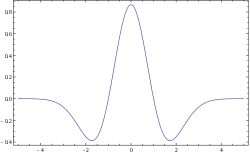
\includegraphics[width=1.0\linewidth]{EDMIIssues/Figures/sombrero.png}
	\end{subfigure}
	\begin{subfigure}{.48\textwidth}
		\centering
		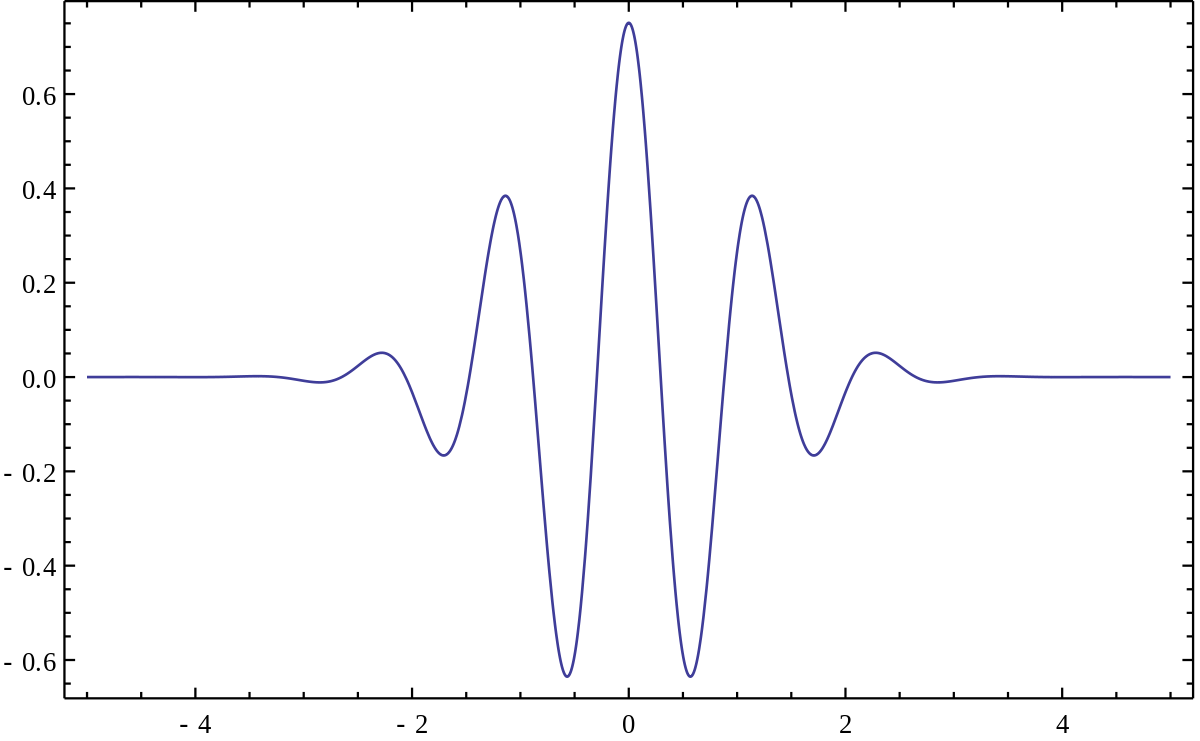
\includegraphics[width=1.0\linewidth]{EDMIIssues/Figures/morlet.png}
	\end{subfigure}
	\caption{Przykładowe falki, po lewej - \textit{sobrero}, po prawej - \textit{morlet}.}
	\label{wavelets}
\end{figure}

$ C(skala, pozycja) = \int f(t) \Psi(skala, pozycja, t) dt $, gdzie: \newline
$ C $ - macierz współczynników, \newline
$ f(t) $ - oryginalny sygnał, \newline
$ \Psi $ - falka.

Dobór skali odbywa się na zasadzie kostki Heisenberga - rozdzielczości czasowa oraz częstościowa zmieniają się, natomiast ich stosunek jest stały.

Ciągła transformacja falkowa zdefiniowana jest jako suma całego omawianego sygnału
pomnożonego przez przeskalowane i przesunięte wersje falki podstawowej:

$ CWT_x^{\Psi^*} (s, \tau) = \int_{-\infty}^{\infty} x(t) \Psi^*_{s, \tau} dt $, gdzie: \newline
$ s $ - skala, \newline
$ \tau $ - przesunięcie (pozycja), \newline
$ x(t) $ - oryginalny sygnał, \newline
$ \Psi^* $ - falka przeskalowana i przesunięta.

$ \Psi^*(s, \tau) = \dfrac{1}{\sqrt{|s|}} \Psi(\dfrac{t- \tau}{s}) $

\underline{Empiryczna analiza modów - EMD}

Funkcja modów własnych spełnia dwa warunki:
\begin{itemize}
	\item Na całej szerokości sygnału liczba przejść przez zero oraz liczba ekstremów musi być, albo jednakowa, albo różnić się maksymalnie o jeden.
	\item W każdym punkcie sygnału średnia wartość obwiedni dolnej oraz górnej wynosi zero.
	\item W $ i $ - tej iteracji 
\end{itemize}

Dekompozycja na mody empiryczne oparta jest na założeniach:\newline
\begin{itemize}
	\item Badany sygnał posiada przynajmniej dwa ekstrema - jedno minimum oraz jedno maksimum.
	\item Charakterystyczna dla sygnału skala czasowa wynika z odstępu między ekstremami.
	\item Jeśli sygnał nie ma żadnych ekstremów, a jedynie punkty przecięcia, można go zróżniczkować jednokrotnie lub wielokrotnie.
\end{itemize}

Procedura "przesiewania" (otrzymywania funckji IMF - \textit{intrinsic mode functions} ) dla metody EMD (rys~\ref{emd}):
\begin{itemize}
	\item Wyznaczyć wszystkie ekstrema sygnału.
	\item Połączyć wszystkie maksyma za pomocą \textit{spline lines} - otrzymujemy obwiednię $ max_i $
	\item To samo dla minimów - otrzymujemy obwiednię $ min_i $
	\item obliczamy średnią $ m_i = \dfrac{min_i + max_i}{2} $
	\item $ h_i = h_{i-1} - m_i $, gdzie $ h_0 = X(t) $. Jeśli w kroku $ i $ prawdziwym będzie kryterium stop np. $ std(h_i, h_{i-1}) < \epsilon $ wtedy nasze $ h_i $ jest modem IMF.
\end{itemize}

\begin{figure} [H]
	\centering
	\begin{subfigure}{.48\textwidth}
		\centering
		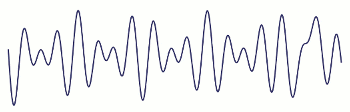
\includegraphics[width=1.0\linewidth]{EDMIIssues/Figures/emd1.png}
	\end{subfigure}
	\begin{subfigure}{.48\textwidth}
		\centering
		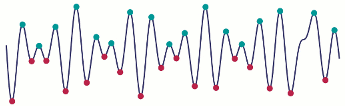
\includegraphics[width=1.0\linewidth]{EDMIIssues/Figures/emd2.png}
	\end{subfigure}
	\begin{subfigure}{.48\textwidth}
		\centering
		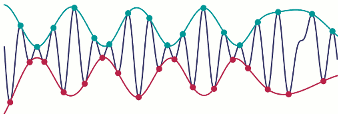
\includegraphics[width=1.0\linewidth]{EDMIIssues/Figures/emd3.png}
	\end{subfigure}
	\begin{subfigure}{.48\textwidth}
		\centering
		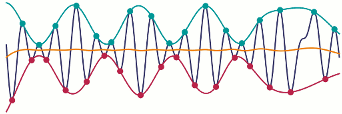
\includegraphics[width=1.0\linewidth]{EDMIIssues/Figures/emd4.png}
	\end{subfigure}
	\caption{Kolejne kroki procedury "przesiewania" dla metody EMD.}
	\label{emd}
\end{figure}

Kolejne mody otrzymujemy poprzez metode przesiewania dla różnicy sygnału oraz znalezionych modów $ r_{k} = X(t) - \sum_{i=0}^{k} c_i $, gdzie $ k $ - liczba znalezionych modów. Jeśli $ r_k $ jest funckją monotoniczną, więcej modów nie może być znalezione - kończymy procedurę.
	
	\subsection{Metody redukcji wymiaru w eksploracji danych.}
	\underline{LDA - \textit{Linear discriminant analysis}} jest używana do znalezienia liniowej kombinacji cech, które najlepiej rozróżniają dwie lub więcej klas obiektów lub zdarzeń. Wynikowe kombinacje są używane jako klasyfikator liniowy lub, częściej, służą redukcji wymiarów do późniejszej klasyfikacji statystycznej. 

Rozważmy zbiór obiektów z których każdy jest opisywany przez wektor cech \textbf{x}, przy czym dla każdego obiektu znana jest jego przynależność do klasy y. Podejście LDA bazuje na założeniu, że funkcje gęstości prawdopodobieństwa $ \forall i \rightarrow p(\textbf{x}|y = i) $ mają rozkłady normalne i jednakowe macierze kowariancji:

$ S = \dfrac{1}{n-1} \sum\limits_{i=1}^{i=n}(x_i - \bar{x})(x_i - \bar{x})^{T} $

LDA próbuje znaleźć podprzestrzeń cech, która maksymalizuje separowalność klas. Dla przypadku dwóch klas oraz dwuwymiarowego wektora cech szukamy takiego kierunku, dla którego rozkłady rzutów zbiorów poszczególnych klas na ten kierunek są jak najbardziej rozdzielone od siebie (rys.~\ref{lda}).

\begin{figure} [H]
	\centering
	\begin{subfigure}{.99\textwidth}
		\centering
		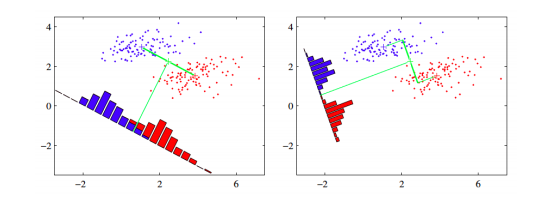
\includegraphics[width=1.0\linewidth]{EDMIIssues/Figures/lda.png}
	\end{subfigure}
	\caption{Przykład LDA.}
	\label{lda}
\end{figure}

\underline{QDA - \textit{Quadratic discriminant analysis}} - zakładamy różne macierze kowarjancji. QDA również próbuje znaleźć podprzestrzeń cech, która maksymalizuje separowalność klas. Dla powyszego przypadku będzie szukać najlepszego rzutu dla rozszerzonego dwuwymiarowego wektora cech o wartości 2-go rzędu tzn. $ [x_1, x_2] \rightarrow [x_1, x_2, x_1^2, x_1x_2, x_2^2] $.

\underline{PCA - Principal components analysis}

\begin{itemize}
	\item zakładamy zbiór wielowymiarowych obserwacji, leżących w przestrzeni $ R^p $,
	\item najczęsciej  obserwacje  nie są  równomiernie  rozrzucone wzdłuż wszystkich kierunków układu współrzędnych,
	\item koncentruj się w pewnych podprzestrzeniach przestrzeni $ R^p $,
	\item kierunki, wzdłuż których znajduje się większość obserwacji, nie muszą się pokrywać z osiami układu współrzędnych $ R^p $,
	\item próba losowa pochodzi z populacji o ciągłym rozkładzie w przestrzeni $ R^p $ z wektorem wartości oczekiwanych \textbf{m} i macierzą kowarjancji \textbf{S}
\end{itemize}

Pierwszą składową główną szukamy poprzez znalezienie takiego kierunku $ \gamma_1 \in R^p $, aby rzut ortogonalny wektora losowego \textbf{x} na ten kierunek dawał zmienną losową o największej warjancji. Kolejne składowe szukamy w ten sam sposób biorąc pod uwagę warunek aby kolejne kierunki były prostopadłe do poprzednich.

Pierwszą składową główną wektora \textbf{x} nazywamy rzut tego wektora na znaleziony kierunek przesunięty o wartość średnią:

$ y_1 = \gamma_1^T(\textbf{x} - \textbf{m}) $

Kolejne składowe główne odpowiadają kolejnym wektorom własnym macierzy kowarjancji \textbf{S}. Pierwsza składowa główna odpowiada wektorowi własnemu o największej wartości własnej ($ \lambda_1 $), kolejne wektory -> kolejne największe wartości własne.

Wielkość:\newline
$ \dfrac{\lambda_1 + ... + \lambda_k}{\lambda_1 + ... + \lambda_p} $\newline
wyraża procent zmienności wektora losowego $ x $ wyjaśnionych przez $ k $ ($ k \le p $) pierwszych składowych głównych.

\underline{Skalowanie wielowymiarowe}

Niech $ d_{ij} $, $ i $, $ j = 1, ..., n $ będą odległościami euklidesowymi między obserwacjami $ \textbf{x}_i $  oraz $ \textbf{x}_j $ w przestrzeni $ R^p $. Zadanie polega na znalezienie takie podprzestrzeni $ R^r $ o wymiarze $ r $, by odległości euklidesowe $ d_{ij}' $ mięszy rzutami obserwacji na tę podprzestrzeń minimalizwowały sumę\newline $ V = \sum\limits_{i=1}^n \sum\limits_{j=1}^n ({d_{ij}}^2 - {d_{ij}'}^2) $

Podobienstwo pomiędzy skalowaniem  wielowymiarowym  ,a  analizą  składowych głównych staje się równoważnością, gdy dana macierz $ d_{ij} $ jest macierzą odległości euklidesowych.

\underline{Autoencoder} - jest rodzajem sztucznej sieci neuronowej wykorzystywanej do uczenia się wydajnego kodowania danych w sposób nienadzorowany. Celem \textit{autoencodera} jest nauczenie się reprezentacji (kodowania) zestawu danych, zazwyczaj w celu zmniejszenia wymiarów, poprzez szkolenie sieci w zakresie ignorowania „szumu” sygnału.

\textbf{Przykład}

Powiedzmy że reprezentujemy zdanie poprzez wektor o długości liczby słów występujących w słowniku. Jeśli słowo występuję w zdaniu, wartość elementu wektora odpowiadającego temu słowu wynosi 1, jeśli słowo występuje dwukrotnie - 2 itd... Słowniki składają się z tysięcy słów, więc nieoptymalna jest reprezentacja zdania w takiej przestrzeni, ponieważ tylko ułamek procenta składowych wektora reprezentującego jakiekolwiek zdanie będzie niezerowych. 

Aby uzyskać reprezentację zdania w mniejszej przestrzeni możemy użyc \textit{autoencodera}. Nasz zbiór uczący przepuszamy przez sieć neuronową gdzie warstwa wejściowa składa się z $ N $(ilość słów w słowniku) neuronów. Warstwa wyjściowa również składa się z $ N $ neuronów. Pomiędzy tymi warstwami jest nieparzysta liczba warstw ukrytych (zazwyczaj symetrycznych), a środkowa warstwa reprezentuje wektor kodujący (rys.~\ref{autoencoder}). Podczas uczenia na wyjściu ustawiamy ten sam wektor co na wejściu.

\begin{figure} [H]
	\centering
	\begin{subfigure}{.99\textwidth}
		\centering
		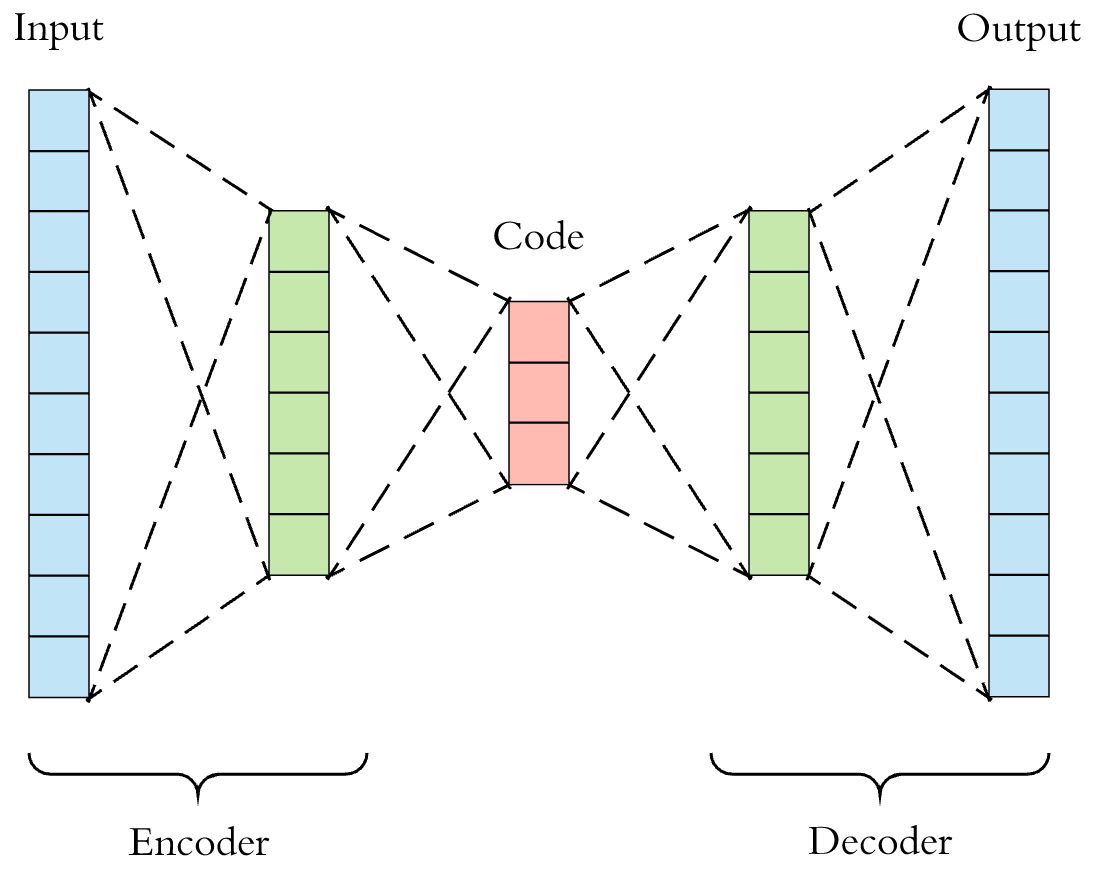
\includegraphics[width=1.0\linewidth]{EDMIIssues/Figures/autoencoder.png}
	\end{subfigure}
	\caption{Topologia sieci neuronowej typu \textit{autoencoder}.}
	\label{autoencoder}
\end{figure}
	
\end{document}
